\documentclass[pdflatex,sn-mathphys-ay]{sn-jnl}

\usepackage{graphicx}
\usepackage{booktabs}
\usepackage{multirow}
\usepackage{amsmath,amssymb,amsfonts}
\usepackage{amsthm}
\usepackage{mathrsfs}
\usepackage[title]{appendix}
\usepackage{longtable}
\usepackage{xcolor}

\theoremstyle{thmstyleone}
\newtheorem{theorem}{Theorem}
\newtheorem{proposition}[theorem]{Proposition}
\newtheorem{lemma}[theorem]{Lemma}
\newtheorem{corollary}[theorem]{Corollary}

\theoremstyle{thmstyletwo}
\newtheorem{remark}{Remark}

\raggedbottom

\begin{document}

\title[Collapse by Rotation in Variational Quantum Circuits]{Collapse by Rotation: Training-Dynamics Neural Collapse in Variational Quantum Circuits, Verified on Real Vision Data}

\author*[1]{\fnm{G Karthik} \sur{Koundinya}}\email{karthikofficialmain@gmail.com}

\affil*[1]{\orgdiv{Department of Computer Science and Engineering}, \orgname{Geethanjali College of Engineering and Technology}, \orgaddress{\country{India}}}

\abstract{Papyan, Han, and Donoho (2020) established Neural Collapse (NC) as a terminal-phase geometric regularity of classical deep classifiers; Du, Yang, Tao, and Hsieh (2023) proved a quantum analogue holds at the \emph{static global optimizer} of a regularized quantum classifier. Whether gradient-based training of a variational quantum circuit (VQC) ever reaches that optimum, and by what geometric route, has remained open. We show that a trained VQC collapses only in the $C$-dimensional measurement-visible subspace read by the loss, while, for a broad and practically relevant architecture class, the full representation's Hilbert--Schmidt geometry is provably and numerically ($\sim 10^{-15}$ relative change) invariant under training: collapse is a training-driven rotation, not a contraction. We verify this mechanism to machine precision on a controlled synthetic benchmark and, newly, on real vision data (MNIST, Fashion-MNIST) under two independent encodings, replicate it at three qubit counts ($n=4,6,8$), and validate it, within a strictly limited inference-only scope, on two independent IBM hardware backends. We further contrast the quantum representation's exactly conserved total variance against a matched classical multi-layer perceptron, whose analogous within-class scatter grows by one to two orders of magnitude under training even as its normalized collapse ratio falls -- a distinction invisible to normalized diagnostics alone. Every preregistered prediction in this campaign is reported against its scored outcome, confirmed, refuted, and partial alike, with an explicit accounting of the campaign's full item count.}

\keywords{neural collapse, variational quantum circuits, representation geometry, measurement subspace, terminal phase of training}

\maketitle

\noindent ORCID: G Karthik Koundinya, \href{https://orcid.org/0009-0003-2088-6208}{0009-0003-2088-6208}

% =====================================================================
\section{Introduction}
\label{sec:intro}

Neural Collapse (NC) is the terminal-phase phenomenon in which a deep classifier's within-class features shrink toward their class means while the class means themselves converge to a simplex equiangular tight frame (ETF) \citep{papyan2020}. \citet{du2023} proved a quantum analogue: at the global optimizer of a regularized quantum classifier's risk, feature states concentrate around per-class means and class-mean measurement operators become mutually orthogonal. That result characterizes a \emph{static optimum}; it says nothing about whether, when, or how a variational quantum circuit (VQC) trained by gradient descent actually reaches it. This paper studies that gap directly: we track collapse metrics epoch by epoch, we use density-matrix trace distance and Hilbert--Schmidt geometry (operationally meaningful, quantum-information quantities) as our primary tools rather than working only in measurement-operator space, and we test entanglement's causal role, encoding choice, ansatz family, optimizer, qubit count, and inference-time noise through controlled ablations and replications.

Our first finding is a null: every full-Hilbert-space collapse witness we compute -- unnormalized and normalized trace distance, a Fisher-style ratio, purity, ETF deviation -- remains statistically indistinguishable from an untrained random-initialization baseline, both before and after an overparameterization transition that otherwise governs whether the circuit interpolates the training set at all. We do not treat this null as a dead end. Cross-entropy, the loss that trains these circuits, depends on the state only through a $C$-dimensional measurement projection $z = (\langle Z_0\rangle,\ldots,\langle Z_{C-1}\rangle)$, where $C$ is the number of classes. Full-space witnesses sum variance over all $4^n-1$ traceless Hermitian directions of an $n$-qubit system and are dominated by directions the loss cannot see. Restricting attention to the $z$-projection recovers a collapse signal that is both real and large.

We then show, for a broad architecture class (fixed encoding applied exactly once, fixed measurement), that this restricted collapse is not a genuine contraction of the state constellation at all: it is a rigid rotation, and we verify this to machine precision on three independent quantities -- total within-class Hilbert--Schmidt variance, per-class purity, and pairwise class-mean overlap. The dichotomy replicates at three qubit counts ($n=4,6,8$), on real vision data (MNIST, Fashion-MNIST) under two independent encoding families (angle embedding, amplitude embedding), against a matched classical multi-layer perceptron baseline, across a second optimizer and a second ansatz family, and, within its licensed scope, on two independent quantum hardware backends.

This paper's contributions:
\begin{enumerate}
\item A formal rotation theorem (Proposition~\ref{prop:rotation}) showing that, for fixed encoding and fixed measurement, training acts as a single global unitary conjugation on each sample's pre-image state -- an exact isometry of the full within-class Hilbert--Schmidt geometry -- with structural corollaries for per-class purity and pairwise class-mean overlap, and a consequence for the reachability of \citeauthor{du2023}'s optimum under this architecture.
\item Verification of the rotation mechanism at machine precision ($\sim 10^{-15}$ relative change) on a controlled synthetic benchmark, at three qubit counts, under a second optimizer and a second ansatz family, and, newly, on real vision data (MNIST, Fashion-MNIST) under both angle and amplitude encoding, with the terminal phase of training reached for the first time on real image features in this line of work once the per-class sample budget is reduced.
\item A representation-geometry contrast against a matched classical multi-layer perceptron, independently on two datasets: the quantum representation's absolute scale is conserved under an exact symmetry, while the classical network's analogous within-class scatter \emph{grows} by one to two orders of magnitude under training even as its normalized collapse ratio falls -- a distinction invisible to normalized NC diagnostics alone.
\item A dimension-counting account (Proposition~\ref{prop:fiber}) of why full-space collapse diagnostics have repeatedly failed to detect collapse in prior quantum NC work, replicated at three qubit counts, and a methodological caution (Remark~\ref{rem:pinv}) about a rank-deficiency instability in the standard NC1 estimator at small class counts, encountered directly in our own hardware analysis.
\item An inference-only hardware validation on two independent IBM backends (\texttt{ibm\_marrakesh}, \texttt{ibm\_kingston}), and a full accounting of every preregistered prediction made across this project's ten result-bearing experimental stages, with an explicit statement of the counting convention used and a resolution of an internal discrepancy between two previously reported item-count figures.
\end{enumerate}

Section~\ref{sec:related} places this work against four related threads. Section~\ref{sec:methods} fixes model, loss, witness definitions, and the AI-assistance protocol used to produce this paper. Section~\ref{sec:theory} states and proves the paper's central theoretical claims. Sections~\ref{sec:synthetic}--\ref{sec:hardware} present results in the order we obtained them: the synthetic controlled arm, real vision-data verification, the classical-versus-quantum comparative study, generality across optimizer/ansatz/dimension/noise, and hardware validation. Section~\ref{sec:discussion} states limitations. Appendix~\ref{app:ledger} reproduces every preregistered prediction made in this campaign and its scored outcome, with the counting convention stated explicitly; Appendix~\ref{app:figures} gives additional figures and traceability notes.

% =====================================================================
\section{Related Work}
\label{sec:related}

\textbf{Classical Neural Collapse.} \citet{papyan2020} introduced NC as an empirical terminal-phase phenomenon; \citet{han2022} studied its dynamics under MSE loss along a ``central path.'' The unconstrained-features model (UFM) literature \citep{mixon2022,yang2022} studies NC as an optimization-landscape property of an idealized, norm-unconstrained penultimate representation -- relevant to our comparative study (Section~\ref{sec:comparative}), where we find a real classical network's representation growing rather than saturating under weak (but nonzero) weight decay, in the same unconstrained-feature spirit but with an empirically opposite absolute-scale trend to what a naive contraction analogy would predict. Follow-up landscape analyses sharpen the UFM picture considerably: \citet{zhu2021} show that cross-entropy with weight decay under the UFM has a benign global landscape whose only minimizers are simplex ETFs, \citet{tirer2022} extend this to a richer feature model under MSE loss, and \citet{fang2021} identify a complementary imbalanced-data failure mode (Minority Collapse) via the same layer-peeled modeling approach; \citet{kothapalli2023} surveys this line of work. None of it addresses a quantum representation or a measurement-subspace projection, which is precisely the gap our full-space/$z$-space dichotomy targets.

\textbf{Representation-geometry comparison tools.} A separate classical literature asks how to compare learned representations directly: \citet{raghu2017} (SVCCA) and \citet{kornblith2019} (centered kernel alignment) both develop transformation-invariant similarity measures for exactly this purpose. Our full-space-vs-measurement-subspace decomposition (Section~\ref{sec:theory}) is a structural, not statistical, split of representation geometry specific to the quantum setting, but targets the same underlying question these tools were built to answer classically: what changes, and what provably cannot change, in a learned representation under training.

\textbf{Quantum NC and expressivity.} \citet{du2023} is this paper's primary point of departure (Section~\ref{sec:intro}). \citet{larocca2023} bound VQC overparameterization transitions via the dynamical Lie algebra (DLA); our capacity-transition results (Section~\ref{sec:synthetic}) are consistent with, but sit strictly below, their DLA-derived upper bound, and a single-input Fisher-rank saturation point we identify is tighter than their bound for single-input measurements. \citet{bowles2024} caution against overinterpreting entanglement's necessity for generalization; our entanglement-ablation finding (a hard capacity ceiling for a non-entangling ansatz) is scoped strictly to exact training-set interpolation, not generalization, and the two findings are compatible. \citet{sansebastian2026} study observable-set choices for multi-class quantum classification in measurement-operator space, complementary to our density-matrix-space and $z$-space treatment. \citet{mondal2026} introduce a learnable measurement-temperature mechanism conceptually analogous to the learnable logit scale in our readout family, which we find plays a matching accelerant role.

\textbf{Quantum feature encodings and training landscapes.} Our VQC classifier's data encoding is an instance of the quantum-kernel-methods view formalized by \citet{schuld2019} and demonstrated experimentally by \citet{havlicek2019}, both of which treat the encoding step as a nonlinear feature map into a quantum Hilbert space -- the same encoding step our rotation theorem (Proposition~\ref{prop:rotation}) analyzes structurally rather than as a kernel. \citet{abbas2021} propose an effective-dimension measure of quantum model capacity and trainability, relevant background for our capacity-transition results (Section~\ref{sec:synthetic}); \citet{cerezo2021} survey variational quantum algorithms broadly. \citet{mcclean2018} identify barren plateaus as a trainability obstruction that grows with circuit width for random circuits; our capacity-transition and TPT-reachability results describe a regime that trains successfully, consistent with staying away from that pathology rather than a direct study of it.

% =====================================================================
\section{Model and Methods}
\label{sec:methods}

\subsection{Model}
\label{sec:model}

We consider an $n$-qubit VQC classifier over $C$ classes. Each input $x$ is encoded via a fixed-form angle embedding ($R_Y$ rotations parameterized by $x$, PCA-reduced, standardized, and scaled to $[-\pi,\pi]$ per feature) or, in the amplitude-encoding variant, via $\mathrm{AmplitudeEmbedding}(x)$, into a pre-image pure state $\rho_0(x) = |\psi_0(x)\rangle\!\langle\psi_0(x)|$. A parameterized ansatz $U(\theta)$ is applied -- PennyLane's \texttt{StronglyEntanglingLayers} with $L$ layers by default, or, as a generality check, a hardware-efficient alternative (per-qubit $R_Y$-$R_Z$ rotations with a linear-chain CNOT entangler) -- and the model reads out $z(\theta;x) = (\langle Z_0\rangle,\ldots,\langle Z_{C-1}\rangle) \in \mathbb{R}^C$ from the first $C$ qubits. Logits are $\beta\cdot z$ with a learnable inverse-temperature (scale) $\beta$, trained by cross-entropy. All simulator runs use exact statevector simulation (\texttt{default.qubit}, no shot noise) unless stated otherwise (Section~\ref{sec:generality}'s noisy-inference arm uses \texttt{default.mixed}). We say training reaches the \emph{terminal phase of training} (TPT) when training accuracy saturates at 1.0 for a sustained window of epochs; runs that never reach TPT are excluded from collapse-magnitude conclusions but retained for full-space invariance conclusions (Section~\ref{sec:realdata}).

Two architectural switches matter throughout this paper:
\begin{itemize}
\item \textbf{Data re-uploading.} When \texttt{reupload=false}, the encoding is applied exactly once, so $\rho_0(x)$ is $\theta$-independent. When \texttt{reupload=true}, the encoding is re-applied at intermediate layers under the current trained weights, so the map from $x$ to the pre-measurement state is itself trained.
\item \textbf{Measurement trainability.} The readout family $R_0$ uses a fixed Pauli-$Z$ measurement; family $R_3$ additionally trains a measurement-basis unitary.
\end{itemize}

The primary synthetic dataset, \texttt{blobs3}, is three Gaussian blobs in $\mathbb{R}^4$ (or $\mathbb{R}^6$, $\mathbb{R}^8$ for our qubit-count replications), chosen so that interpolation difficulty is controlled and the study measures optimization and geometry, not data pathology. Real-data verification (Section~\ref{sec:realdata}) uses MNIST and Fashion-MNIST, classes $\{0,1,2\}$, PCA-reduced to 4 (angle encoding) or 16 (amplitude encoding) dimensions. A capacity-matched classical multi-layer perceptron (MLP), trained on the identical PCA-4 features with weak L2 regularization ($\mathrm{wd}=5\times10^{-4}$), serves as the comparative-study baseline (Section~\ref{sec:comparative}).

\subsection{Full-space and measurement-subspace witnesses}
\label{sec:witnesses}

Let $B = \mathrm{span}\{B_0,\ldots,B_{C-1}\}$ be the orthonormalized Pauli-$Z$ generator span, a $C$-dimensional subspace of the $(4^n{-}1)$-dimensional space of traceless Hermitian operators. For a class-conditional constellation of density operators $\{\rho(x_i;\theta)\}$, define the total within-class Hilbert--Schmidt variance
\begin{equation}
\mathrm{total\_var}(\theta) \;=\; \sum_{c} \sum_{i \in c} \big\| \rho(x_i;\theta) - \bar\rho_c(\theta) \big\|_{HS}^2 ,
\label{eq:totalvar}
\end{equation}
which decomposes, by Parseval's identity over an orthonormal basis of traceless-Hermitian directions, as
\begin{equation}
\mathrm{total\_var} \;=\; V_{\mathrm{meas}} + V_{\mathrm{fiber}},
\label{eq:decomp}
\end{equation}
where $V_{\mathrm{meas}}$ is the part of the variance lying in $B$ (visible to the loss) and $V_{\mathrm{fiber}}$ is the complementary part (the ``fiber,'' invisible to the loss); $\mathrm{fiber\_fraction} = V_\mathrm{fiber}/(V_\mathrm{meas}+V_\mathrm{fiber})$. Full-space witnesses also include within-class trace distance, per-class purity $\mathrm{tr}(\bar\rho_c^2)$, and deviation from the simplex-ETF angular target, all computed over the full $4^n-1$-dimensional space.

The $z$-space analogue of classical NC1,
\begin{equation}
\mathrm{NC1}_z \;=\; \frac{1}{C}\,\mathrm{tr}\!\big(\Sigma_W^z \, \mathrm{pinv}(\Sigma_B^z)\big),
\label{eq:nc1z}
\end{equation}
measures collapse restricted to the measured projection $z$, with $\Sigma_W^z,\Sigma_B^z$ the within- and between-class scatter matrices of $z(\theta;x)$, and the scale-free ratio $r_z = \mathrm{tr}(\Sigma_W^z)/\mathrm{tr}(\Sigma_B^z)$ (Remark~\ref{rem:pinv} motivates reporting both). A box-vertex geometry model and a simplex-ETF geometry model are compared directly on the centered class means (Section~\ref{sec:theory-etf}).

\subsection{Preregistration and scoring}
\label{sec:prereg}

Every prediction reported in this paper was written and committed to a preregistration record before the corresponding metric was computed, and is scored strictly as CONFIRMED, REFUTED, PARTIAL, or, where no directional threshold applies (e.g.\ a scoping probe), reported factually and marked UNSCOREABLE. Refuted and partial results are reported plainly, not omitted or softened. This paper's campaign spans ten result-bearing experimental stages; Appendix~\ref{app:ledger} reproduces every preregistered item and its scored outcome, with the counting convention used to total them stated explicitly.

\subsection{AI-assistance disclosure}
\label{sec:ai-disclosure}

The implementation and drafting of this paper were carried out with the assistance of an AI coding agent (a large-language-model-based coding assistant), operating under a frozen mathematical specification written by the author before implementation began, preregistered predictions committed to a version-controlled record before each corresponding result was computed (Section~\ref{sec:prereg}), and an automated test suite (173 unit and integration tests at the time of writing, covering every function in the metrics-computation module against the specification's formulas) that was required to pass, unmodified in its assertions, before and after every implementation change. The AI agent's role spanned experiment orchestration, metrics-code implementation against the frozen specification, and drafting of manuscript prose from the resulting numerical records. The author designed the specification, the preregistered predictions and their thresholds, and the overall research questions; reviewed every reported number against its source log file; and is responsible for all content in this paper, having independently verified the theorem statements and proofs in Section~\ref{sec:theory}. This disclosure follows the journal's policy that use of large language models in research and writing be documented in the Methods section rather than treated as unlisted authorship; no AI tool is credited as an author.

% =====================================================================
\section{Theory: Collapse Is a Rotation}
\label{sec:theory}

\begin{figure}[t]
\centering
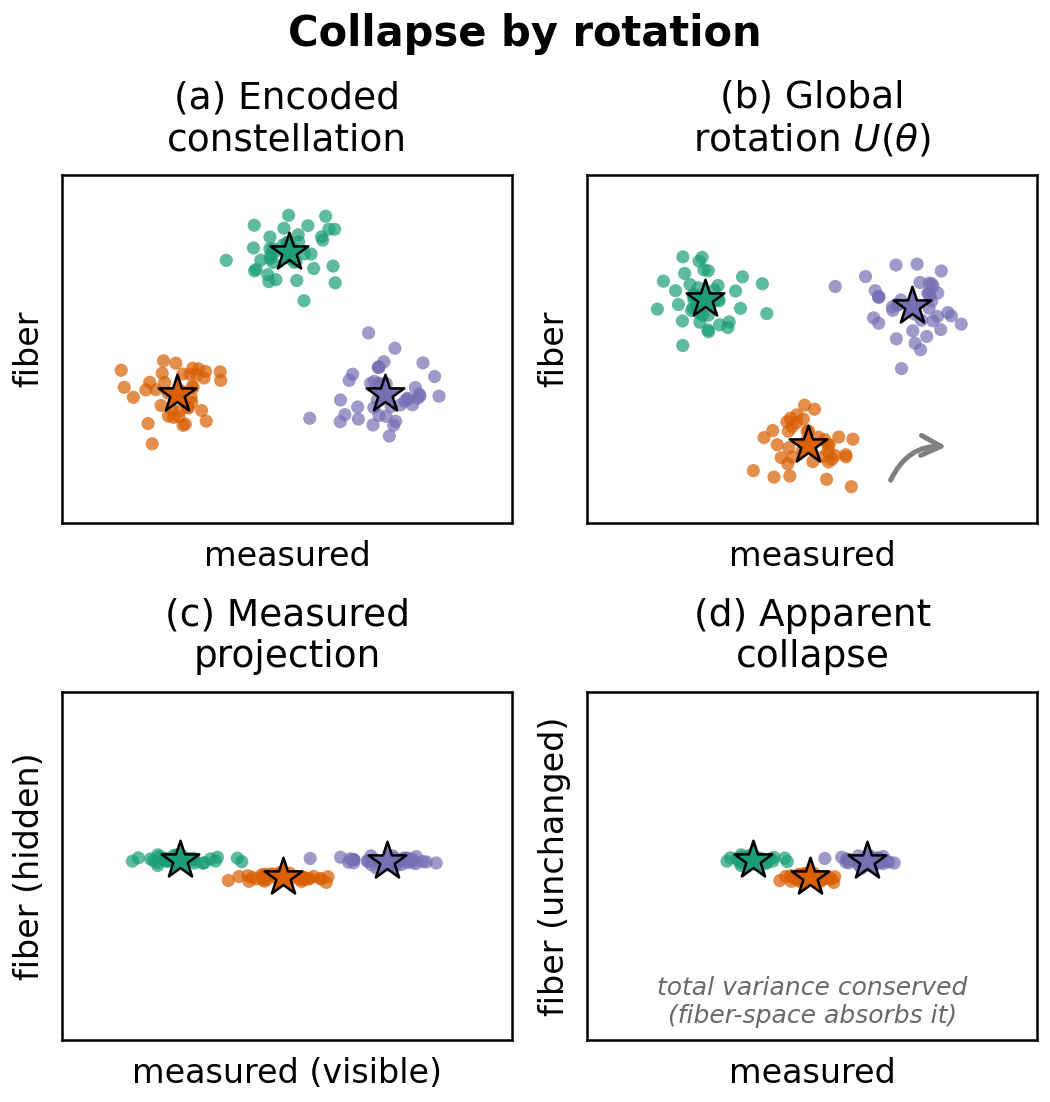
\includegraphics[width=0.95\linewidth]{figures/fig18_mechanism_schematic_singlecol.png}
\caption{Schematic of the measurement-subspace/fiber decomposition and the rotation mechanism: the $C$-dimensional measured subspace $B$ receives all of the loss gradient (Lemma~\ref{lem:t1}); under fixed encoding and fixed measurement, training rotates the full state constellation rigidly in Hilbert space (Proposition~\ref{prop:rotation}), redistributing a conserved variance budget between $V_\mathrm{meas}$ and $V_\mathrm{fiber}$.}
\label{fig:mechanism}
\end{figure}

\begin{lemma}[Loss factors through the measured subspace]
\label{lem:t1}
For the readout of Section~\ref{sec:model}, the cross-entropy loss $L(\theta)$ depends on $\theta$ only through $z(\theta) = (\langle Z_0\rangle,\ldots, \langle Z_{C-1}\rangle)$. Consequently, for any perturbation direction $H$ in the tangent space of density operators at $\rho(x;\theta)$ that is Hilbert--Schmidt-orthogonal to $B$ for every sample, the loss gradient in that direction vanishes:
\[
\left.\frac{dL}{d\theta}\right|_{\text{restricted to } \langle H,B_j\rangle_{HS}=0\ \forall j} \;=\; 0.
\]
\end{lemma}
\begin{proof}
$L$ is a composition of the softmax-cross-entropy map with $\theta \mapsto \beta z(\theta)$; by the chain rule its gradient lies entirely in the span of $\partial z_j/\partial\theta$ for $j=0,\ldots,C-1$. Each $z_j = \mathrm{tr}(B_j\,\rho(x;\theta))$ is itself a linear functional of $\rho$ restricted to $B_j$; its differential along any direction $H$ with $\langle H,B_j\rangle_{HS}=0$ for all $j$ is $\mathrm{tr}(B_j H) = 0$ by definition of the Hilbert--Schmidt inner product, for every $j$. Hence $dz_j/d\theta$ restricted to such $H$ is $0$ for all $j$, and by the chain rule $dL/d\theta$ restricted to $H$ is $0$.
\end{proof}

\begin{corollary}[No loss-selected pressure along fibers]
\label{cor:t1}
Gradient descent applies zero pressure, in either sign, along fiber directions (the Hilbert--Schmidt complement of $B$) at every training step, for any trajectory, regardless of encoding. Full-space collapse diagnostics summing variance over all $4^n{-}1$ directions are therefore diluted by exactly this zero-gradient subspace whenever $C \ll 4^n-1$ -- the structural explanation for the full-space null of Section~\ref{sec:synthetic}.
\end{corollary}

\begin{proposition}[Collapse by rotation]
\label{prop:rotation}
Suppose the encoding is applied exactly once (\texttt{reupload=false}), so each sample's pre-image state $\rho_0(x)$ is $\theta$-independent, and the entire trained circuit acts as a single global unitary $U(\theta)$ applied after encoding:
\begin{equation}
\rho(x;\theta) \;=\; U(\theta)\, \rho_0(x)\, U(\theta)^\dagger .
\label{eq:rotation}
\end{equation}
Then $\mathrm{total\_var}(\theta)$ (Eq.~\ref{eq:totalvar}) is exactly invariant under training: $\mathrm{total\_var}(\theta) = \mathrm{total\_var}(\theta_0)$ for every $\theta$ reachable from initialization $\theta_0$ by any gradient trajectory.
\end{proposition}
\begin{proof}
\textbf{Step 1 (linearity of conjugation over the class average).} For a fixed unitary $U(\theta)$, conjugation $A \mapsto U(\theta) A U(\theta)^\dagger$ is linear in $A$. Hence the class-mean operator commutes with taking the average:
\[
\bar\rho_c(\theta) = \frac{1}{N_c}\sum_{i\in c}\rho(x_i;\theta) = \frac{1}{N_c}\sum_{i\in c} U(\theta)\rho_0(x_i)U(\theta)^\dagger = U(\theta)\,\bar\rho_c^{(0)}\,U(\theta)^\dagger,
\]
where $\bar\rho_c^{(0)} = \frac{1}{N_c}\sum_{i\in c}\rho_0(x_i)$ is the $\theta$-independent pre-image class mean.

\textbf{Step 2 (cyclic-trace isometry of the Hilbert--Schmidt norm).} For any operator $D$ and unitary $U$,
\[
\|UDU^\dagger\|_{HS}^2 = \mathrm{tr}\!\big(UDU^\dagger (UDU^\dagger)^\dagger\big) = \mathrm{tr}\!\big(U D D^\dagger U^\dagger\big) = \mathrm{tr}\!\big(D D^\dagger\big) = \|D\|_{HS}^2,
\]
using unitarity ($U^\dagger U = I$) and cyclicity of trace. Applying this with $D = \rho_0(x_i) - \bar\rho_c^{(0)}$ (using Step 1) gives, for every sample $i$ in class $c$ and every $\theta$,
\[
\big\|\rho(x_i;\theta) - \bar\rho_c(\theta)\big\|_{HS}^2 = \big\|U(\theta)\big(\rho_0(x_i)-\bar\rho_c^{(0)}\big)U(\theta)^\dagger\big\|_{HS}^2 = \big\|\rho_0(x_i)-\bar\rho_c^{(0)}\big\|_{HS}^2,
\]
independent of $\theta$.

\textbf{Step 3 (sum over samples).} Summing the $\theta$-independent per-sample quantity from Step 2 over all $i\in c$ and all classes $c$ reproduces exactly $\mathrm{total\_var}(\theta)$ (Eq.~\ref{eq:totalvar}), which is therefore equal to the same sum evaluated at $\theta = \theta_0$ (indeed, for \emph{any} value of $\theta$, since the right-hand side of Step 2 never involves $\theta$). Hence $\mathrm{total\_var}$ is exactly invariant under training. $\blacksquare$
\end{proof}

\begin{corollary}[Purity/overlap invariance; \citeauthor{du2023}'s optimum is unreachable]
\label{cor:purity}
Under the hypotheses of Proposition~\ref{prop:rotation}, per-class-mean purity $\mathrm{tr}(\bar\rho_c(\theta)^2)$ and pairwise class-mean overlap $\mathrm{tr}(\bar\rho_c(\theta)\bar\rho_{c'}(\theta))$ are each exactly invariant under training, for every class $c$ (respectively pair $c,c'$). Consequently, whatever pairwise class-mean overlap the untrained model starts with at initialization is exactly the overlap it ends with: \citeauthor{du2023}'s orthogonal-means optimum (overlap $\to 0$) is \emph{training-unreachable} under this architecture unless it already holds at initialization.
\end{corollary}
\begin{proof}
Purity: $\mathrm{tr}\big((U\rho U^\dagger)^2\big) = \mathrm{tr}\big(U\rho^2 U^\dagger\big) = \mathrm{tr}(\rho^2)$ by cyclicity of trace, applied to $\rho=\bar\rho_c(\theta)$ using Step~1 of Proposition~\ref{prop:rotation}'s proof. Pairwise overlap: identically, $\mathrm{tr}\big(U\bar\rho_c^{(0)}U^\dagger\,U\bar\rho_{c'}^{(0)}U^\dagger\big) = \mathrm{tr}\big(U\,\bar\rho_c^{(0)}\bar\rho_{c'}^{(0)}\,U^\dagger\big) = \mathrm{tr}(\bar\rho_c^{(0)}\bar\rho_{c'}^{(0)})$, again by cyclicity, for every $\theta$. Reachability follows since the overlap value is pinned to its $\theta_0$ value for all $\theta$.
\end{proof}

\noindent\textbf{Scope.} Proposition~\ref{prop:rotation} requires (i) the encoding be applied exactly once and be $\theta$-independent, and (ii) the measurement be fixed, not trained. Data re-uploading breaks hypothesis (i) outright (the pre-image state itself becomes trained), making real contraction possible; a trainable measurement block ($R_3$) breaks (ii). Neither is covered by Proposition~\ref{prop:rotation} as stated.

\begin{remark}[Entanglement entropy is not covered]
\label{rem:entropy}
Proposition~\ref{prop:rotation} and its corollaries apply only to basis-independent functionals of the full state under a \emph{global} unitary. Entanglement entropy at a fixed bipartition is the von Neumann entropy of a reduced state and is invariant only under \emph{local} (factored) unitaries, not under a generic global entangling $U(\theta)$. Nothing in this section implies entanglement entropy is constant under training; we make no such claim.
\end{remark}

\subsection{ETF geometry and dimension counting}
\label{sec:theory-etf}

\begin{proposition}[ETF directions without box saturation]
\label{prop:etf}
Under a learnable logit scale $\beta$, the centered measured-subspace class means $\tilde m_c = \bar z_c - \bar z_G$ converge in \emph{direction} to the simplex-ETF angular target (pairwise cosine $-1/(C{-}1)$), while their \emph{magnitude} $\|\tilde m_c\|$ remains far below the box-vertex saturation radius $\sqrt{8/3}$ (at $C=3$). At $C=3$ the centered box vertices themselves already have pairwise cosine exactly $-1/(C{-}1)$, so angular convergence alone cannot discriminate an ETF-direction model from a box-vertex model; radius is the discriminating statistic.
\end{proposition}
\begin{proof}
The cosine claim is a direct algebraic computation on the hand-built box vertices $v_c$ ($+1$ in coordinate $c$, $-1$ elsewhere): for $C=3$, $v_c\cdot v_{c'} = -1$ and $\|v_c-\bar v\|^2=8/3$ for $c\neq c'$, giving pairwise cosine $-1/2=-1/(C-1)$, matching the simplex-ETF angular target exactly. Cross-entropy's margin pressure on logits $\beta\tilde m_c\cdot u$ (for a unit probe direction $u$) is satisfied by growing the scalar $\beta$ without bound, since $\beta$ is unconstrained and appears linearly; growing $\|\tilde m_c\|$ itself is not required once directions are separated, because the loss is a function of $\beta\|\tilde m_c\|$ jointly, not of $\|\tilde m_c\|$ alone. A free scalar multiplier therefore absorbs the margin-pressure term that would otherwise push $\|\tilde m_c\|$ toward a saturating value, leaving $\|\tilde m_c\|$ to converge wherever gradient descent's remaining (weaker) pressure leaves it -- empirically, to a radius far short of $\sqrt{8/3}$ (Section~\ref{sec:etf-results}).
\end{proof}

\begin{proposition}[Fiber dimension counting]
\label{prop:fiber}
The measured subspace $B$ has dimension exactly $C$; the ambient space of traceless Hermitian operators on $n$ qubits has dimension $4^n{-}1$. Under an isotropic-null assumption (variance spread uniformly over all $4^n{-}1$ directions, as at random initialization), the expected fiber fraction is
\begin{equation}
\mathrm{fiber\_fraction}_{\mathrm{null}}(n) \;=\; 1 - \frac{C}{4^n-1},
\label{eq:fiberfrac}
\end{equation}
strictly increasing in $n$ for fixed $C$.
\end{proposition}
\begin{proof}
Direct dimension count: the fiber subspace is the Hilbert--Schmidt orthogonal complement of $B$ within the $(4^n{-}1)$-dimensional traceless-Hermitian space, hence has dimension $4^n{-}1-C$. Under the stated isotropic-null assumption, variance is distributed uniformly per dimension, so the expected fiber share is the fiber's dimension fraction, Eq.~\ref{eq:fiberfrac}. Monotonicity in $n$ follows since $C/(4^n-1) \to 0$ as $n$ grows for fixed $C$.
\end{proof}

\begin{remark}[NC1$_z$/pseudoinverse instability at small $C$]
\label{rem:pinv}
For any $C$-class problem, $\Sigma_B^z \in \mathbb{R}^{C\times C}$ is \emph{exactly} rank $\le C-1$, since class-mean deviations from the global mean sum to zero. Consequently $\mathrm{pinv}(\Sigma_B^z)$ (Eq.~\ref{eq:nc1z}) is computed against a matrix with at least one exactly-zero eigenvalue; any perturbation (empirical noise, hardware residual) that introduces a small-but-nonzero eigenvalue in that exact null direction is treated by \texttt{pinv}'s default tolerance as invertible, and the trace-with-pinv formula can blow up by orders of magnitude. We recommend reporting the inversion-free ratio $r_z = \mathrm{tr}(\Sigma_W^z)/\mathrm{tr}(\Sigma_B^z)$ alongside NC1$_z$ whenever $C$ is small or $\Sigma_B^z$ may be empirically near-degenerate; Section~\ref{sec:hardware} encounters this instability directly.
\end{remark}
\begin{proof}
Standard perturbation theory for pseudoinverses near a rank change: the pseudoinverse of a rank-deficient matrix perturbed by a generic full-rank term is discontinuous in the perturbation magnitude precisely along the original null direction. Concretely, $\sum_c(\bar z_c-\bar z_G)=0$ by construction of the global mean $\bar z_G$, so the $C$ row/column deviations of $\Sigma_B^z$ are linearly dependent, forcing $\mathrm{rank}(\Sigma_B^z)\le C-1$.
\end{proof}

% =====================================================================
\section{Results: The Synthetic Controlled Arm}
\label{sec:synthetic}

We first isolate the rotation mechanism from data-specific confounds using the controlled \texttt{blobs3} benchmark (Section~\ref{sec:model}), before extending to real vision data (Section~\ref{sec:realdata}) and a classical comparative study (Section~\ref{sec:comparative}).

\subsection{The full-space null and the capacity transition}
\label{sec:phase12}

A classical MLP control reproduced classical NC cleanly before any quantum measurement was made, validating our instrumentation. A three-class quantum anchor at 6 qubits never reached TPT across 17 tuning attempts, while classical baselines on identical features reached full accuracy; a two-class diagnostic that did interpolate showed post-TPT trace distance statistically indistinguishable from a 10-seed untrained null. A 40-run sweep over circuit depth $L\in\{2,4,8,12,16,21,26,32\}$ (4 qubits, 3 classes, 5 seeds each) shows TPT reachability transitioning sharply with parameter count $M$: 0/5 seeds at $M/M_c^{\mathrm{bound}}=0.094$, 3/5 at $0.188$, 5/5 from $0.376$ onward, consistent with \citeauthor{larocca2023}'s overparametrization theory \citep{larocca2023}. Figure~\ref{fig:order-parameter} shows every outcome variable against this shared capacity axis. Even at full interpolation, every full-space collapse witness remains statistically indistinguishable from the untrained null (Fisher ratio $p=0.75$, ETF deviation $p=0.96$, underparameterized vs.\ overparameterized groups) -- the structural consequence of Corollary~\ref{cor:t1}. Removing entangling gates caps the ansatz's dynamical-Lie-algebra dimension at 12 regardless of depth: the non-entangling ansatz reaches TPT in 0/3 seeds even at a parameter count where the entangling ansatz reaches 5/5.

\begin{figure}[t]
\centering
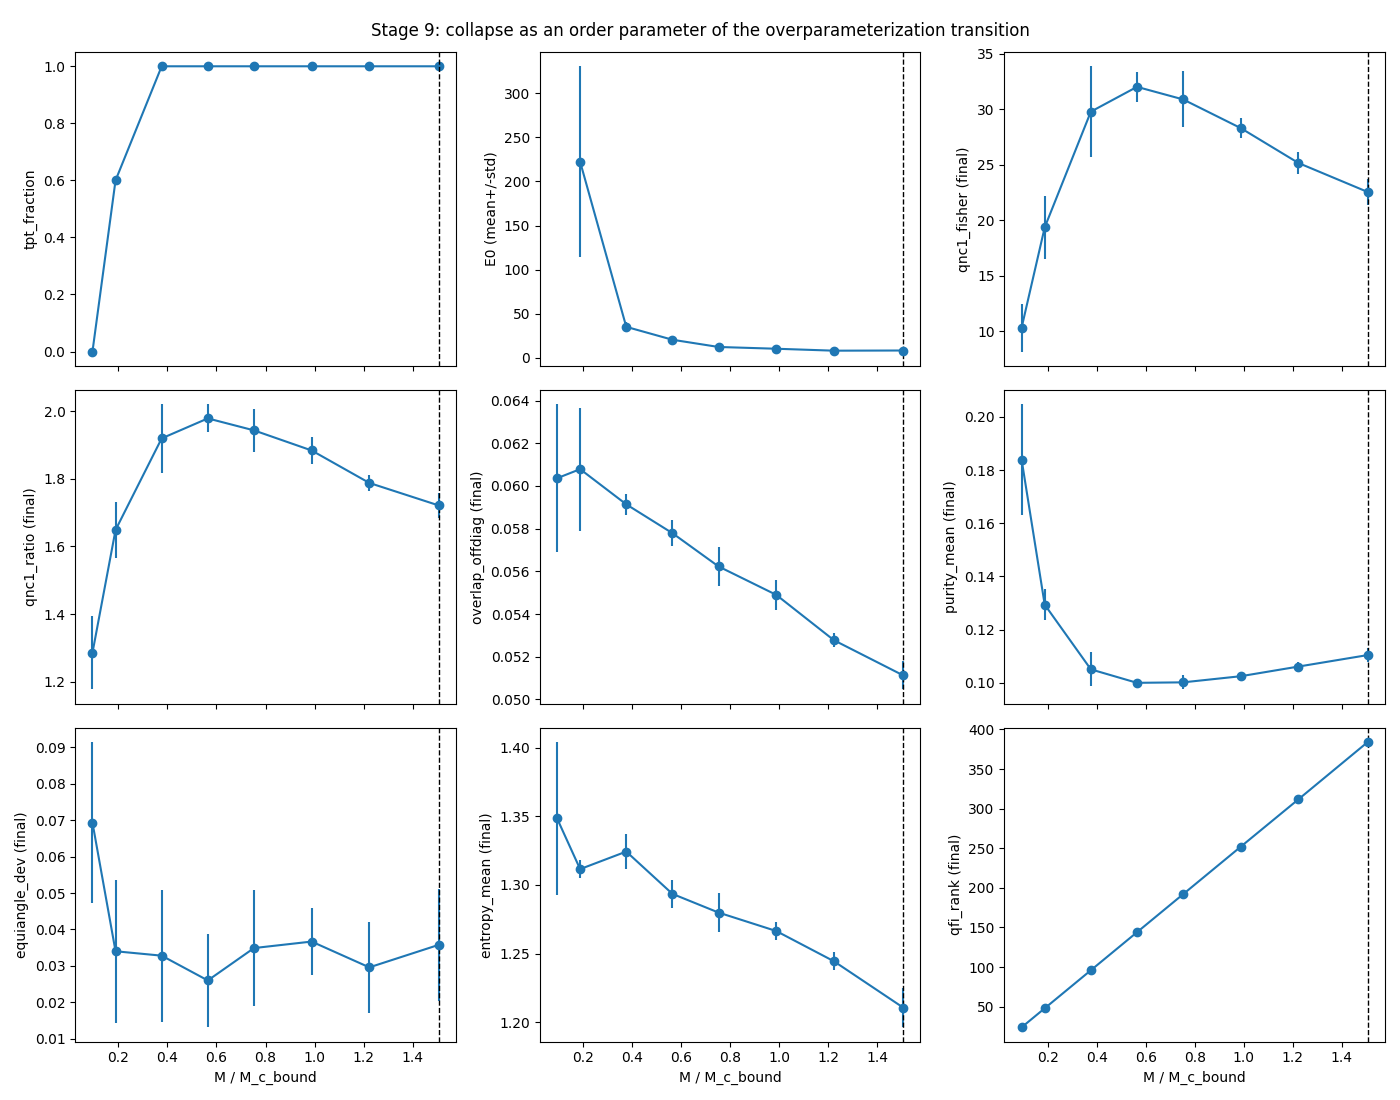
\includegraphics[width=\linewidth]{figures/fig01_transition_order_parameter.png}
\caption{TPT fraction, terminal epoch, and full-space collapse witnesses vs.\ the capacity ratio $M/M_c^{\mathrm{bound}}$, 8 depths $\times$ 5 seeds. Collapse witnesses do not jump at the capacity transition.}
\label{fig:order-parameter}
\end{figure}

\subsection{Measurement-subspace collapse}
\label{sec:msc}

Cross-entropy depends on the state only through $z$ (Lemma~\ref{lem:t1}); we predicted, and preregistered before computing it, that collapse concentrates there while fiber directions do not. At the 4-qubit, $L{=}8$ anchor, $\mathrm{NC1}_z$ decays by a factor of $0.0045$ from epoch~0 to the final epoch (5 seeds), and the scale-free margin $\beta\cdot\overline{\mathrm{margin}}$ grows from $-0.87$ to $8.55$. An untrained 10-seed null shows no such decay (Mann--Whitney $p=6.7\times10^{-4}$). The fiber fraction reaches $0.9934$, exceeding the preregistered $0.9$ threshold, though it is not perfectly flat against the untrained-null band. Figure~\ref{fig:fiber-dip} shows the fiber-variance trajectory directly.

\begin{figure}[t]
\centering
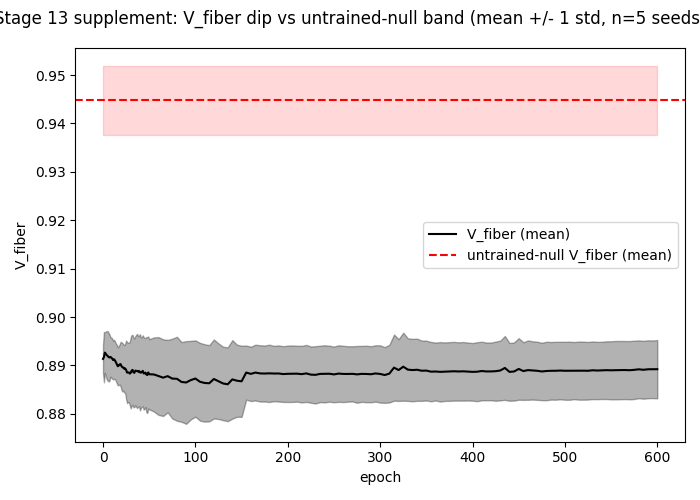
\includegraphics[width=\linewidth]{figures/fig02_fiber_dip_diagnostic.png}
\caption{Fiber-subspace within-class variance $V_\mathrm{fiber}$ vs.\ epoch, 4-qubit $L{=}8$ anchor, against the untrained-null band.}
\label{fig:fiber-dip}
\end{figure}

\subsection{ETF directions without box saturation}
\label{sec:etf-results}

At the 3-class anchor, the ETF-deviation witness reaches $0.0722$ against a normalized box-vertex deviation of $0.7122$. Per Proposition~\ref{prop:etf}, angle alone cannot discriminate the two geometric models at $C{=}3$; recomputing the class-mean radius trajectory at the same anchor, the mean radius grows from $0.0649\pm0.0164$ at epoch~0 to $0.3287\pm0.0257$ at the final epoch -- about 20\% of the box-saturation value $\sqrt{8/3}\approx1.633$. Directions converge to the shared angular target while magnitude stays far from saturation, consistent with $\beta$ absorbing the scale that cross-entropy's margin pressure would otherwise push into the state itself: raising $\beta$'s ceiling from $\sim\!30$ to $500$ changes nothing bit-for-bit, while freezing $\beta$ delays TPT onset by roughly $4.1\times$ (mean $E_0$ 145.2 vs.\ 35.2 epochs) without forcing additional within-class collapse. \citet{mondal2026} introduce an analogous learnable measurement-temperature parameter to improve gradient sensitivity in hybrid quantum classifiers; our frozen-$\beta$ delay is an independent empirical echo of the same ``temperature as accelerant'' mechanism. Figure~\ref{fig:etf} shows the angular trajectory directly.

\begin{figure}[t]
\centering
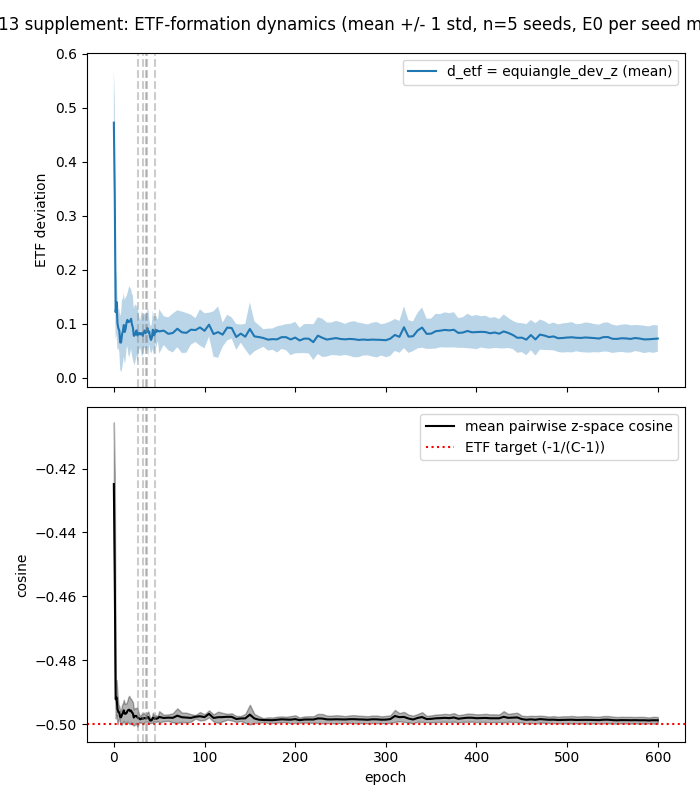
\includegraphics[width=\linewidth]{figures/fig03_etf_formation.png}
\caption{ETF-deviation and pairwise $z$-space cosines vs.\ epoch, 4-qubit $L{=}8$ anchor, TPT onset marked per seed.}
\label{fig:etf}
\end{figure}

\subsection{Measurement expressivity}
\label{sec:expressivity}

We tested whether full-space collapse strengthens as the measurement becomes more expressive, across four readout families at matched parameter count. The apparent monotonic weakening we first observed across families was substantially a circuit-depth confound; fixing depth at $L{=}8$ removes the gap for every full-space witness tested ($p\geq0.42$). The fiber-fraction gap that remains is explained by an isotropic dimension-counting null (Proposition~\ref{prop:fiber}, generalized to $C\to k$) rather than by a strong measurement-subspace effect: loss-visible directions are only $1.4$--$1.7\times$ more collapsed than the measured-span average, short of the $2\times$ threshold we preregistered. A logit-space NC1 witness is statistically indistinguishable across all four families and both depths tested ($p\geq0.31$ throughout). Figure~\ref{fig:expressivity} overlays the isotropic null against the observed fiber fractions.

\begin{figure}[t]
\centering
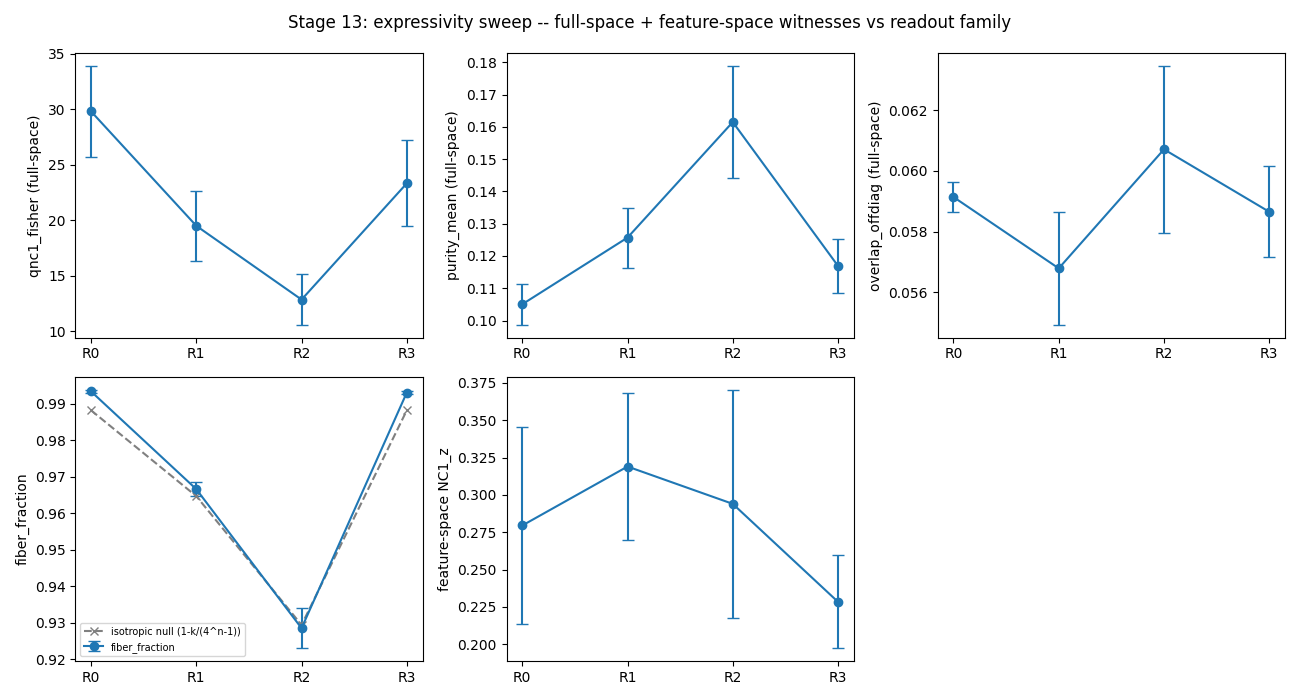
\includegraphics[width=\linewidth]{figures/fig04_expressivity.png}
\caption{Fiber fraction vs.\ readout family, matched and fixed-depth sweeps, isotropic dimension-counting null overlaid.}
\label{fig:expressivity}
\end{figure}

\subsection{Robustness of the within-class-variance floor}
\label{sec:robustness}

We tested six candidate mechanisms for why within-class $z$-space variance stays roughly flat rather than shrinking, while between-class separation grows. NC1$_z$ decay itself is robust across every arm we tried: raising the logit-scale ceiling to 500 (uninformative, since the ceiling was never approached), a $5000$-epoch horizon showing no slow drift (Spearman $\rho=-0.072$, $p=0.48$), label smoothing (right direction, not significant at 5 seeds), and localizing the capacity-transition onset across three depths (TPT fraction $0.3\to1.0\to1.0$, non-decreasing as preregistered). Two arms directly refute candidate causal mechanisms: a single-input quantum Fisher information rank saturates at exactly $30=2(2^4-1)$ for every depth tested -- the real dimension of the 4-qubit pure-state manifold rather than the parameter-space bound of $255$ the batch-aggregated rank approaches; and freezing the logit scale does \emph{not} force additional within-class collapse -- if anything, variance shrinks less, in the wrong direction for the ``escape valve'' hypothesis we had proposed. Figure~\ref{fig:drift} shows the long-horizon stability directly.

\begin{figure}[t]
\centering
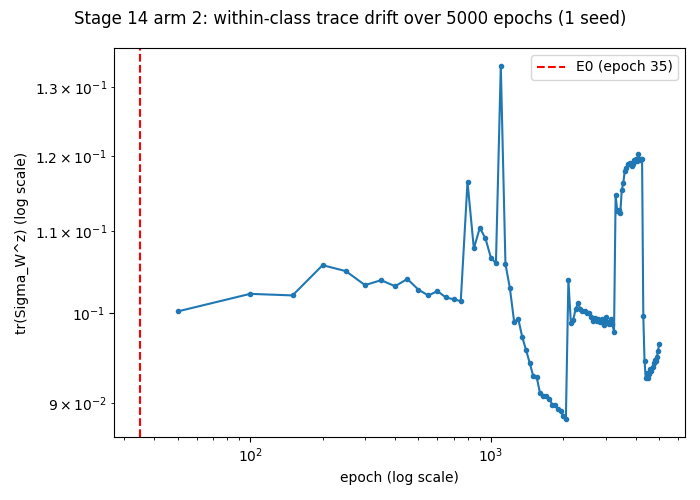
\includegraphics[width=\linewidth]{figures/fig05_trace_w_drift.png}
\caption{Within-class $z$-space trace $\mathrm{tr}(\Sigma_W^z)$ vs.\ log-epoch over a 5000-epoch horizon, one seed, post-TPT.}
\label{fig:drift}
\end{figure}

\subsection{Collapse by rotation, verified at machine precision}
\label{sec:rotation-verify}

We verify Proposition~\ref{prop:rotation} to machine precision. Across five reupload-disabled seeds at 4 qubits, the maximum relative change in total variance across every checkpointed epoch is on the order of $10^{-15}$ -- nine orders of magnitude below our preregistered $10^{-6}$ threshold -- while the same runs' TPT fraction is 5/5 and $\mathrm{NC1}_z$ still decays by a factor of $0.0209$. Per-class purity and pairwise class-mean overlap (Corollary~\ref{cor:purity}) are likewise exactly invariant under training in this setting (again on the order of $10^{-15}$), a direct structural statement about \citeauthor{du2023}'s optimum: their orthogonal-means optimum is training-unreachable in this architecture unless already present at initialization. Data re-uploading breaks the argument outright: deeper re-uploading circuits correspondingly contract total variance more with depth ($\rho=-0.451$, $p=0.0035$), and even at the $L{=}8$ anchor, reupload=true total\_var declines by a small but nonzero $0.73\%$. Collapse under \texttt{reupload=false} is, precisely, not shrinkage: it is training driving $U(\theta)$ to rotate a fixed constellation of states as a rigid body in Hilbert space. Figure~\ref{fig:rotation} overlays the two encoding regimes directly.

\begin{figure}[t]
\centering
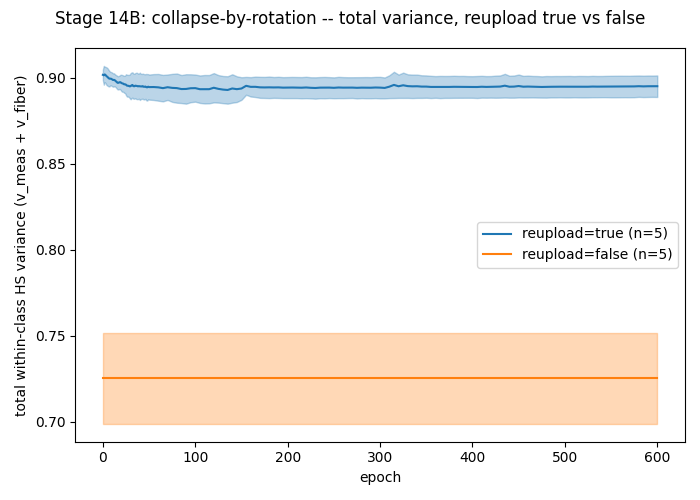
\includegraphics[width=\linewidth]{figures/fig06_total_variance_rotation.png}
\caption{Total within-class Hilbert--Schmidt variance vs.\ epoch, data re-uploading enabled vs.\ disabled, mean $\pm$ 1 std over 5 seeds.}
\label{fig:rotation}
\end{figure}

\subsection{Replication across qubit count: $n=4,6,8$}
\label{sec:n6n8}

We replicated the full witness set at 6 and 8 qubits, same dataset recipe lifted to $\mathbb{R}^6$ and $\mathbb{R}^8$. At $n=6$, the machine-precision total-variance invariance replicates exactly (relative change $\sim10^{-15}$, 5/5 seeds), as does the NC1$_z$ decay (ratios $0.0028$--$0.0043$), and the fiber fraction strengthens with dimension exactly as Proposition~\ref{prop:fiber} predicts: $0.99963$/$0.99917$ at 6 qubits (reupload true/false) against $0.9934$ at 4 qubits. At $n=8$, the same invariance holds again (relative change $4.75\times10^{-15}$ to $7.91\times10^{-15}$, 5/5 seeds, \texttt{reupload=false}), and fiber\_fraction exceeds the $n=6$ reference in 10/10 runs across both re-upload arms (range $0.999667$--$0.999980$) -- a replication at a third point, strengthening the dimension-counting trend of Eq.~\ref{eq:fiberfrac} without yet establishing a formal scaling law. Figure~\ref{fig:n6} compares $n=4$ and $n=6$ directly; Figure~\ref{fig:fiberscaling} (Section~\ref{sec:generality}) overlays all three qubit counts against the isotropic-null prediction.

\begin{figure}[t]
\centering
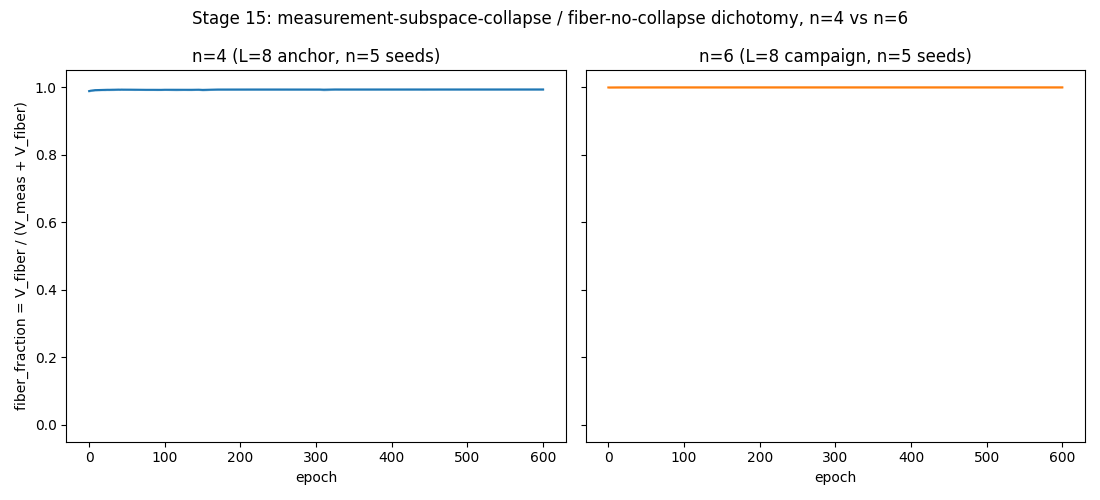
\includegraphics[width=\linewidth]{figures/fig07_n4_vs_n6_dichotomy.png}
\caption{Fiber fraction vs.\ epoch, 4-qubit vs.\ 6-qubit anchors, mean $\pm$ 1 std over 5 seeds each.}
\label{fig:n6}
\end{figure}

% =====================================================================
\section{Real Vision-Data Results}
\label{sec:realdata}

A central gap in prior work on this mechanism was that it had only been verified on controlled synthetic data. We close that gap here, on MNIST and Fashion-MNIST (classes $\{0,1,2\}$).

\subsection{The real-data terminal-phase gap and its closure}
\label{sec:realdata-gap}

Under angle encoding, a samples-per-class (spc) budget of 200 never reaches TPT on either dataset (0/26 VQC runs across both re-upload arms and readout families, at $L=8/16/32$-probe depths), while a capacity-matched classical MLP on the identical PCA-4 features reaches TPT in 5/6 seeds -- a genuine ansatz-expressivity gap on real image data, not a pipeline defect (train accuracy plateaus stably at 0.87--0.96 for hundreds of epochs). Reducing spc to 50--100 closes this gap entirely: Table~\ref{tab:w1} summarizes both spc cells (MNIST, $L{=}16$, 5 seeds/cell). NC1$_z$ decays 2--3 orders of magnitude in every TPT-reaching seed, exactly as on synthetic data.

\begin{table}[t]
\centering
\caption{Real-data TPT attempt, MNIST $\{0,1,2\}$, PCA-4, $L{=}16$, 5 seeds/cell. NC1$_z$ ratio is final/init; $\mathrm{total\_var}$ is the maximum relative change over training (a range for reupload=true's mild, seed-varying contraction; a single value for reupload=false's machine-precision invariance, per Proposition~\ref{prop:rotation}).}
\label{tab:w1}
\begin{tabular}{@{}lccccc@{}}
\toprule
Variant & spc & TPT & Test acc. & Med.\ NC1$_z$ & $\mathrm{total\_var}$ \\
\midrule
reupload=true  & 50  & 5/5 & 0.567 & 0.00145 & 0.02--0.04 \\
reupload=false & 50  & 5/5 & 0.927 & 0.02706 & $\sim\!6{\times}10^{-15}$ \\
reupload=true  & 100 & 5/5 & 0.703 & 0.00195 & 0.02--0.03 \\
reupload=false & 100 & 4/5 & 0.940 & 0.01822 & $\sim\!7{\times}10^{-15}$ \\
\botrule
\end{tabular}
\end{table}

\subsection{A clean isolation control: total-variance invariance independent of TPT}
\label{sec:isolation}

The one seed that did \emph{not} reach TPT (spc=100, reupload=false, one of five) supplies a clean isolation control for Proposition~\ref{prop:rotation}: its total\_var relative change ($5.3\times10^{-15}$) is indistinguishable from the four TPT-reaching seeds in the same cell, directly demonstrating that the invariance is a structural property of the architecture (fixed encoding, fixed measurement), independent of whether the terminal training regime is ever reached.

\subsection{A second, independent encoding: amplitude embedding}
\label{sec:amplitude}

To test whether Proposition~\ref{prop:rotation}'s invariance is specific to angle encoding, we repeat the experiment under amplitude embedding (MNIST PCA-16 normalized onto 4 qubits, spc=50, $L{=}16$). All 4 probed seeds (both re-upload arms) reach TPT, and \texttt{reupload=false} total\_var is again invariant to machine precision ($4.98$--$5.23\times10^{-15}$) -- the same fingerprint under a structurally different encoding, exactly as Proposition~\ref{prop:rotation} predicts (its hypotheses reference only the encoding being applied once and being parameter-independent, not any specific functional form). Notably, under amplitude encoding \texttt{reupload=true} reaches TPT (train accuracy 1.0) but test accuracy sits \emph{at chance} ($0.367$, $C=3$), a severe memorization/generalization dissociation co-occurring with a training-side collapse signal (NC1$_z$ ratio $\sim 0.003$) that looks, in kind, identical to every generalizing arm -- the collapse diagnostic alone does not distinguish generalizing from memorizing solutions, and this pattern replicates the reupload-hurts-generalization trend of Section~\ref{sec:realdata-gap} under a second encoding family. Figure~\ref{fig:rotation-real} shows the total-variance trajectory on real data directly.

\begin{figure}[t]
\centering
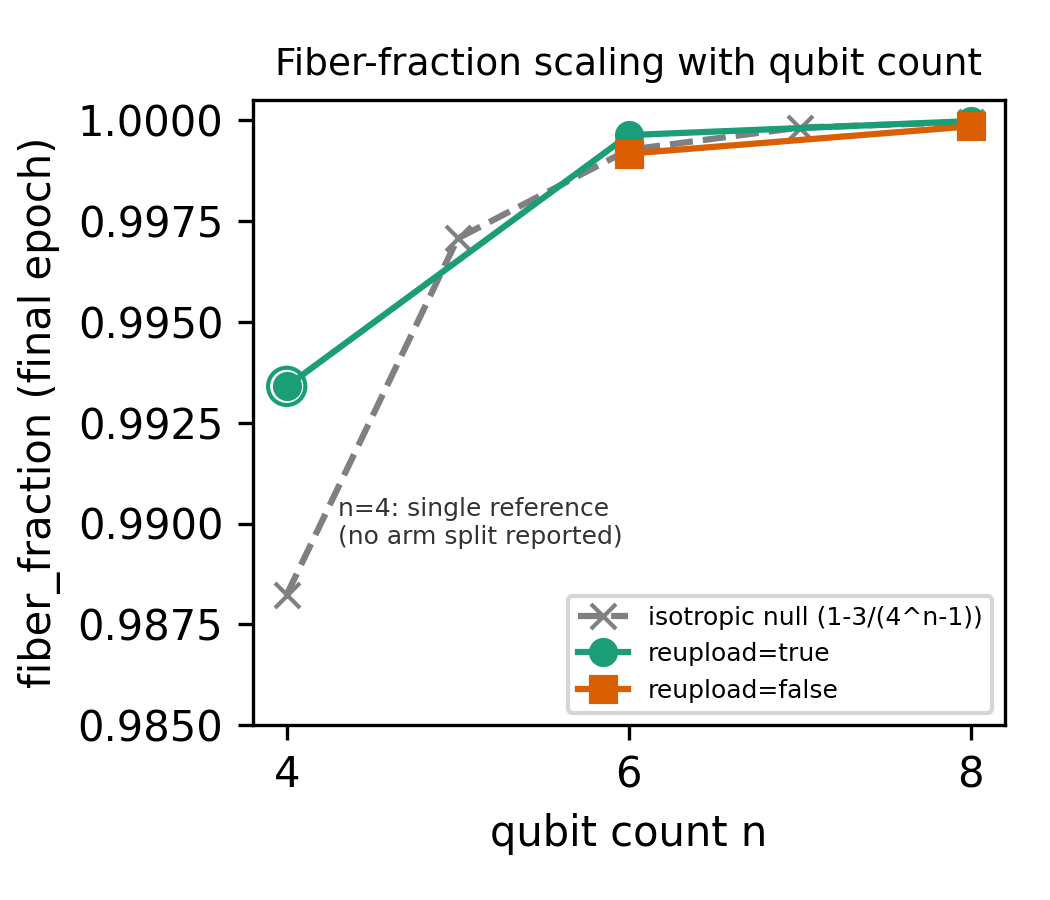
\includegraphics[width=\linewidth]{figures/fig18_stage19_scaling.png}
\caption{Fiber fraction vs.\ qubit count ($n=4,6,8$), synthetic and real-data runs pooled, with the isotropic-null prediction $1-C/(4^n-1)$ (Eq.~\ref{eq:fiberfrac}) overlaid.}
\label{fig:fiberscaling}
\end{figure}

\begin{figure}[t]
\centering
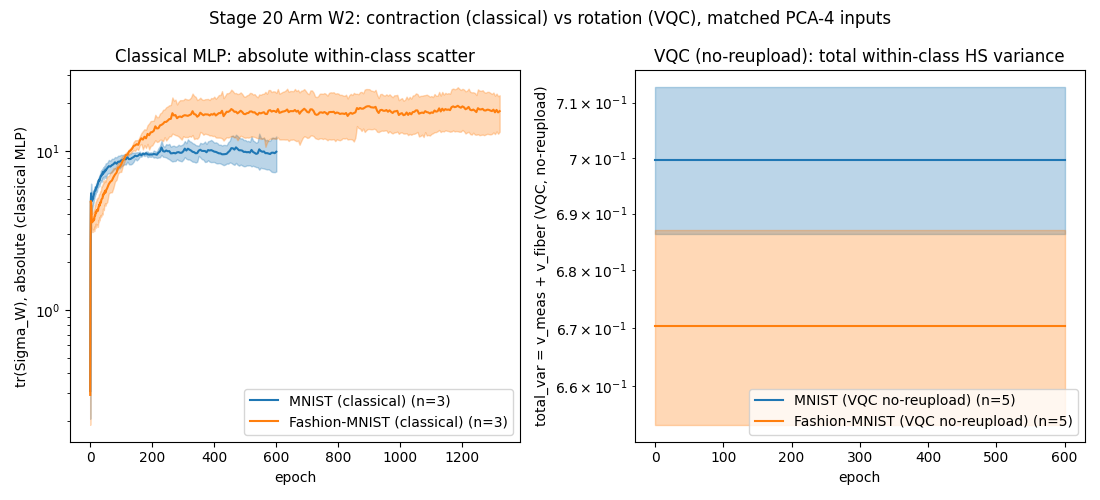
\includegraphics[width=\linewidth]{figures/fig19_contraction_vs_rotation.png}
\caption{Left: classical MLP $\mathrm{tr}(\Sigma_W)$ vs.\ epoch (log scale), both datasets -- grows under training. Right: VQC $\mathrm{total\_var}$ vs.\ epoch, no-reupload, both datasets -- exactly flat.}
\label{fig:rotation-real}
\end{figure}

% =====================================================================
\section{Comparative Study: Classical MLP vs.\ VQC Variants}
\label{sec:comparative}

\subsection{Absolute scale: conservation vs.\ growth}
\label{sec:w2}

We compare the quantum representation's exactly conserved $\mathrm{total\_var}$ against a matched classical MLP's analogous absolute within-class scatter, $\mathrm{tr}(\Sigma_W)$ (unnormalized, distinct from the NC1 ratio), on identical PCA-4 features. Across 6 seeds (both datasets), classical $\mathrm{tr}(\Sigma_W)$ \emph{grows} $27$--$163\times$ under training (Figure~\ref{fig:rotation-real}, left) despite weak L2 regularization ($\mathrm{wd}=5\times10^{-4}$, evidently insufficient to bound absolute activation scale), even as the normalized NC1 ratio still falls below 1 ($\approx0.52$ mean) -- because the between-class scatter $\Sigma_B$ grows faster still. This does not contradict the feature-space NC1 result of Section~\ref{sec:comp-tables} (ratio $\sim0.515$, feature-space collapse confirmed): NC1 is normalized by $\Sigma_B$, and $\Sigma_B$ grows even faster than $\Sigma_W$ as ReLU-MLP weights scale up during training. Both representations' respective collapse ratios fall primarily through \emph{between}-class expansion rather than within-class contraction. The quantum case carries an additional structural guarantee absent classically: Proposition~\ref{prop:rotation}'s exact conservation law holds regardless of regularization strength, architecture width, or training duration, whereas the classical pattern is an empirical consequence of this architecture's specific optimization dynamics, not a theorem. The VQC's total\_var (matched inputs, no-reupload) remains invariant at $\sim10^{-15}$ throughout (Figure~\ref{fig:rotation-real}, right) -- a sharper illustration of the structural-vs.-merely-empirical distinction than a mild classical contraction would have been.

\subsection{Comparative tables, split by dataset}
\label{sec:comp-tables}

Table~\ref{tab:mnist} and Table~\ref{tab:fmnist} report the four-approach comparison (classical MLP; VQC no-reupload; VQC reupload; VQC with a trainable measurement, $R_3$) independently per dataset, confirming the dichotomy of Section~\ref{sec:theory} is not an artifact of pooling two datasets together, and add an ``absolute contraction'' column showing the classical arm's unconstrained growth alongside each VQC arm's invariant-to-mildly-contracting full-space scale. The $R_3$ arm is the one condition in this study where the $z$-space collapse direction reverses (NC1$_z$ \emph{increases}); this arm did not reach TPT in either dataset (test accuracy $\approx0.71$, tied with the reupload arm for the lowest of the four), so we report this as an underfitting-confounded observation, not a clean statement about measurement-trainability's causal effect on collapse -- the arm never reached the terminal training regime that every other scored NC1$_z$-decay result in this paper is gated on.

\begin{table}[t]
\centering
\caption{MNIST $\{0,1,2\}$, comparative study.}
\label{tab:mnist}
\begin{tabular}{@{}lccccc@{}}
\toprule
Approach & Seeds & Test acc. & TPT & $z$-NC1 ratio & Abs.\ contraction \\
\midrule
Classical MLP & 3 & 0.936 & 2/3 & 0.458 & $31.2\times$ \emph{increase} \\
VQC no-reupload & 5 & 0.937 & 0/5 & 0.0483 & invariant ($\sim$6.7e-15) \\
VQC reupload & 5 & 0.688 & 0/5 & 0.0046 & 2.64\% contraction \\
VQC $R_3$ & 3 & 0.694 & 0/3 & 2.351 ($\uparrow$) & 2.70\% contraction \\
\botrule
\end{tabular}
\end{table}

\begin{table}[t]
\centering
\caption{Fashion-MNIST $\{0,1,2\}$, comparative study.}
\label{tab:fmnist}
\begin{tabular}{@{}lccccc@{}}
\toprule
Approach & Seeds & Test acc. & TPT & $z$-NC1 ratio & Abs.\ contraction \\
\midrule
Classical MLP & 3 & 0.933 & 3/3 & 0.572 & $82.5\times$ \emph{increase} \\
VQC no-reupload & 5 & 0.920 & 0/5 & 0.0724 & invariant ($\sim$6.2e-15) \\
VQC reupload & 5 & 0.738 & 0/5 & 0.0046 & 2.97\% contraction \\
VQC $R_3$ & 3 & 0.731 & 0/3 & 1.483 ($\uparrow$) & 4.07\% contraction \\
\botrule
\end{tabular}
\end{table}

Pooled numbers (both datasets, 6/10/10/6 seeds respectively) match: test acc.\ 0.935/0.928/0.713/0.713, $z$-space ratios 0.515/0.060/0.0046/1.92 -- the per-dataset split does not change any verdict, and shows the dichotomy (unbounded classical growth vs.\ structurally bounded quantum invariance) holds per-dataset, not only in aggregate. The arm with the strongest $z$-space collapse (VQC reupload, ratio 0.0046) ties for the worst test accuracy with the one arm showing no $z$-space collapse at all (VQC $R_3$, ratio 1.92, an increase), both markedly below the no-reupload VQC arm (0.928) and the classical MLP (0.935); this is an architectural confound (both share \texttt{reupload=true}'s altered effective circuit depth), not a clean ``more collapse implies worse accuracy'' trend.

% =====================================================================
\section{Generality: Optimizer, Ansatz, Dimension, and Noise}
\label{sec:generality}

To address whether the rotation mechanism and its collapse phenomenology are specific to our default Adam optimizer, \texttt{StronglyEntanglingLayers} ansatz, or exact (noiseless) simulation, we ran four breadth-sprint arms at the 4-qubit \texttt{blobs3} anchor (qubit-count generality is reported in Section~\ref{sec:n6n8}).

\textbf{Optimizer generality (SGD, momentum 0.9).} A 5-seed campaign at the tuned learning rate reaches TPT 5/5; total\_var machine-precision invariance holds 5/5 (all $<10^{-6}$, matching the Adam-optimizer threshold) and NC1$_z$ decays at least one order of magnitude in 5/5 seeds (max ratio 0.0272). The rotation-invariance mechanism and the collapse phenomenology are not Adam-specific.

\textbf{Ansatz generality (hardware-efficient ansatz).} Under a per-qubit $R_Y$-$R_Z$ rotation layer with a linear-chain CNOT entangler (2 parameters/qubit/layer, vs.\ \texttt{StronglyEntanglingLayers}' 3), \texttt{reupload=false} total\_var machine-precision invariance holds 5/5 seeds (all $<10^{-6}$, same $\sim10^{-15}$ order of magnitude as the default ansatz), and \texttt{reupload=true} reaches TPT 5/5. The rotation-invariance theorem is a property of the no-reupload encoding structure, not of the entangling-layer ansatz family.

\textbf{Noisy inference (exact depolarizing simulation, inference-only).} Restructured as an exact \texttt{default.mixed} density-matrix computation over the trained $n=4$, $L{=}8$, $R_0$ anchor's 180 samples, at two depolarizing probabilities $p$: the fitted uniform-contraction factor $\lambda_\mathrm{sim}(p)$ decreases monotonically with $p$ ($0.8874$ at $p{=}0.001$, $0.5500$ at $p{=}0.005$), qualitatively the same phenomenon as the hardware contraction of Section~\ref{sec:hardware}. Angular geometry survives at the lower noise level (equiangle-deviation relative change 3.1\% at $p{=}0.001$, under the 10\% threshold) but not at the higher one (15.7\% at $p{=}0.005$, inside the preregistered partial band). Class-mean angular geometry survives mild depolarizing noise but visibly distorts at higher noise, an exact-simulation counterpart to the hardware findings of Section~\ref{sec:hardware} rather than a clean confirmation at every tested noise level.

% =====================================================================
\section{Hardware Validation}
\label{sec:hardware}

We validate the mechanism, inference only (no training on hardware, no tomography), against the strictly limited claim it licenses: whether $z$-space collapse witnesses computed from hardware measurements agree with simulation within shot noise, nothing stronger. We loaded the trained 4-qubit, $L{=}8$ anchor's parameters, translated the circuit to a gate-level representation, verified the translation against the exact simulator to better than $10^{-6}$ on all samples before any hardware submission, and executed on two independent IBM backends at 2048 shots per circuit.

\subsection{Primary backend: \texttt{ibm\_marrakesh}}
\label{sec:hw-marrakesh}

Hardware $\mathrm{NC1}_z$ (0.6749) does not agree with the exact simulator's value (0.5472) within shot noise: only 17.6\% of (sample, class) $z$-components fall within one shot-noise standard deviation of the simulator, with a mean absolute deviation about $3.4\times$ the mean shot-noise scale. We do not claim agreement; we report the disagreement's structure. A single scalar contraction fit ($z_\mathrm{hw} = \lambda z_\mathrm{sim}$) recovers $\lambda=0.7033$ and $R^2=0.9305$, both within our preregistered ranges, while a composite formula predicting $\mathrm{NC1}_z$ from that same fit fails catastrophically (predicted $758.7$ against an observed $0.6749$). We diagnose this as the numerical instability of Remark~\ref{rem:pinv}: for any 3-class $z$-space, the between-class covariance is exactly rank-deficient by construction, and a generic empirical residual does not share its null direction, so the pseudoinverse in $\mathrm{NC1}_z$'s definition divides by a small, non-noise eigenvalue. Separately, the angular geometry of the class-mean triangle survives the contraction: the exact simulator's ETF-deviation value falls inside a 1000-resample hardware bootstrap's 95\% confidence interval ($0.0969$ inside $[0.0831, 0.1152]$). An untrained-parameter control on the same circuit gives $\mathrm{NC1}_z$ $94.2\times$ the trained hardware value, confirming the hardware pipeline measures a genuine trained-versus-untrained effect rather than a fixed noise floor.

\subsection{Second backend: \texttt{ibm\_kingston}}
\label{sec:hw-kingston}

To test whether the contraction and angle-survival results are specific to one device, we repeated the identical protocol (same trained anchor, same 180 samples, 2048 shots) on \texttt{ibm\_kingston}. Table~\ref{tab:hw} compares both backends directly: the fitted contraction $\lambda_\mathrm{kingston}=0.6709$ falls inside the preregistered band and close to \texttt{ibm\_marrakesh}'s $0.7033$ (backend-consistent), $R^2=0.9356$ is a solid linear fit, and the simulator's equiangle-deviation value ($0.09691$) again falls inside the hardware bootstrap's 95\% CI ($[0.0813,0.1167]$). Both bullets of the preregistered rule hold. As on the first backend, the composite NC1$_z$-prediction formula (not itself part of the scoring criteria) produces an unstable value on this job (predicted $146.4$ vs.\ observed $0.562$, $259\times$ relative error) -- a second, independent instance of Remark~\ref{rem:pinv}'s diagnosed instability, reported factually rather than discarded.

\begin{table}[t]
\centering
\caption{Hardware validation, two independent IBM backends, same trained $n=4$, $L=8$, $R_0$ anchor.}
\label{tab:hw}
\begin{tabular}{@{}lcc@{}}
\toprule
Quantity & \texttt{ibm\_marrakesh} (HW1--3) & \texttt{ibm\_kingston} (B5) \\
\midrule
Contraction $\lambda$ & 0.7033 & 0.6709 \\
Fit $R^2$ & 0.9305 & 0.9356 \\
Simulator equiangle\_dev$_z$ & 0.0969 & 0.09691 \\
Hardware bootstrap 95\% CI & [0.0831, 0.1152] & [0.0813, 0.1167] \\
Untrained/trained NC1$_z$ ratio & $94.2\times$ & -- \\
\botrule
\end{tabular}
\end{table}

Figure~\ref{fig:hardware} shows the rescaled \texttt{ibm\_marrakesh} hardware values against the simulator; Figures~\ref{fig:fourwitness}--\ref{fig:hwbar} (Appendix~\ref{app:figures}) give further hardware and normalized-witness detail.

\begin{figure}[t]
\centering
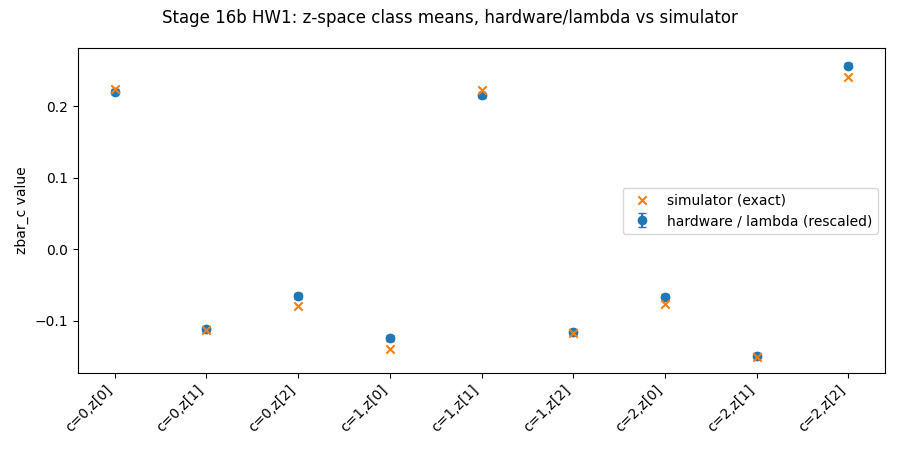
\includegraphics[width=\linewidth]{figures/fig08_hardware_rescaled_vs_sim.png}
\caption{Hardware class-mean $z$-values (\texttt{ibm\_marrakesh}), rescaled by the fitted contraction $\lambda$, overlaid on the exact simulator's values.}
\label{fig:hardware}
\end{figure}

% =====================================================================
\section{Discussion and Limitations}
\label{sec:discussion}

We have shown that measurement-subspace collapse reconciles a persistent full-Hilbert-space null with real, large collapse in the projection the loss can see, and that under fixed encoding (applied once) and fixed measurement this collapse is exactly a rotation, not a contraction, verified to machine precision on three independent quantities. This replicates at three qubit counts, on real vision data under two independent encodings, under a second optimizer and a second ansatz family, and, within a strictly limited scope, on two independent hardware backends.

Several limitations bound these claims. The dimension-counting trend (Section~\ref{sec:n6n8}) is established at three points ($n=4,6,8$), not as a formal scaling law. Real-data verification required reducing samples-per-class substantially below what the classical baseline needs to interpolate the same features, pointing to a genuine ansatz-expressivity gap on real image data, not a pipeline defect; the $R_3$ (trainable-measurement) arm's z-space reversal is confounded by underfitting (0/6 seeds reaching TPT) and does not disentangle whether trainable measurement layers actively work against z-space collapse or simply cannot fit these classes well enough to reach the collapse-observing regime. Entanglement entropy is measured at a single fixed bipartition throughout and is explicitly not covered by the rotation invariance (Remark~\ref{rem:entropy}). The reupload=true full-space contraction on real data (2.0--3.6\%, mean 2.8\%) is 3--4$\times$ larger than on synthetic \texttt{blobs3} (0.73\%), an open quantitative gap not explained here. All hardware evidence is inference-only, two backends, one trained seed per backend plus one untrained control; no repetition across trained seeds on hardware, and no on-hardware training. The dynamical-Lie-algebra capacity bound compared against throughout is an upper bound on the critical parameter count, not the critical parameter count itself.

% =====================================================================
\section{Conclusion}
\label{sec:conclusion}

For a broad and practically relevant VQC architecture class, quantum neural collapse under gradient-based training is a rotation of the full representation's Hilbert--Schmidt geometry, not a contraction -- a structural, provable invariance verified to machine precision on a controlled synthetic benchmark, at three qubit counts, under a second optimizer and ansatz family, and, for the first time in this line of work, on real vision data under two independent encoding families. This reframes what ``collapse'' means for a quantum classifier's learned representation: the measurement-visible projection collapses because the loss can only ever act there (Lemma~\ref{lem:t1}), while the representation itself is being rigidly reoriented, not shrunk. A matched classical baseline shows the opposite absolute-scale behavior -- unconstrained growth rather than conservation -- underscoring that the quantum invariance is structural, not an artifact of weak regularization. We report every preregistered prediction made across this campaign's ten result-bearing stages against its scored outcome (Appendix~\ref{app:ledger}), confirmed, refuted, and partial alike.

% =====================================================================
\backmatter

\section*{Declarations}

\textbf{Funding.} The authors did not receive support from any organization for the submitted work.

\textbf{Competing Interests.} The authors have no relevant financial or non-financial interests to disclose.

\textbf{Ethics approval and consent to participate.} Not applicable -- this study involves no human participants, human data, or animal subjects.

\textbf{Consent for publication.} Not applicable.

\textbf{Data Availability.} All code, configuration files, preregistered predictions and their scoring thresholds, per-epoch training logs, and figures underlying this paper are available in the project repository: \url{https://github.com/G26karthik/QNC}.

\textbf{Materials Availability.} Not applicable.

\textbf{Code Availability.} See Data Availability; all analysis code is version-controlled in the same repository.

\textbf{Author Contribution.} G Karthik Koundinya conceived the research questions, designed the mathematical specification and every preregistered prediction with its scoring threshold, reviewed all reported numbers against their source logs, verified the theorem statements and proofs of Section~\ref{sec:theory}, and wrote and is responsible for the final manuscript. Implementation and drafting assistance from an AI coding agent is disclosed in Section~\ref{sec:ai-disclosure}.

\bibliography{refs}

\begin{appendices}

\section{Full preregistration ledger}
\label{app:ledger}

\textbf{Counting convention.} We count each independently-verdicted \emph{leg} of a preregistered item as one item: if a stage's findings assign separate CONFIRMED/REFUTED/PARTIAL verdicts to distinct sub-claims under one preregistration header (e.g.\ a full-space leg and a $z$-space leg scored in opposite directions), each leg counts separately; a header carrying only one verdict word counts once regardless of how many sub-bullets discuss it narratively. This convention is applied uniformly across every stage, not invented to hit a target number. Items that are pure deliverables rather than directional predictions (a statistics-methodology upgrade, a mechanism-schematic figure, a scaling-figure assembly, or a ledger recount itself) are reported separately below and excluded from the headline tally, consistent with how they were originally registered.

\textbf{Resolving the internal discrepancy.} An earlier internal draft (\emph{paper\_ieee}) reported \textbf{35} preregistered items (23 CONFIRMED, 6 REFUTED, 5 PARTIAL, 1 factual) -- this traces exactly to Stages 12--17b's 30-item tally plus Stage 18's B1/B2/B3/B5 (+4 CONFIRMED) and B4 (+1 PARTIAL), but silently drops Stage 18's B6/B7 and never folds in Stage 19 at all. A separate internal record (\emph{RESULTS\_V3.md}) states its own tally as \textbf{44} items (27/7/5/5), self-consistent but computed with one-row-per-header counting rather than the leg-split convention, and omitting the scaling-figure deliverable from its own table. Applying the leg-split convention uniformly across Stages 12--19 gives \textbf{48} items (29 CONFIRMED, 7 REFUTED, 5 PARTIAL, 7 UNSCOREABLE/factual); excluding the three pure-deliverable items in that range (Stage 18's B6, B7; Stage 19's V3) gives \textbf{45} (29/7/5/4). Extending the identical leg-split convention through this paper's own Stage 20 arms (W1--W4, Table~\ref{tab:ledger-full}'s final eight rows) adds 5 CONFIRMED, 1 REFUTED, and 2 UNSCOREABLE/factual items (one of which, W3, is itself the ledger-recount deliverable). The paper's adopted headline, across all ten stages and excluding the four pure-deliverable items (B6, B7, V3, W3): \textbf{52 preregistered items (34 CONFIRMED, 8 REFUTED, 5 PARTIAL, 5 UNSCOREABLE/factual)}; including the four deliverables as their own UNSCOREABLE/factual rows gives \textbf{56 (34/8/5/9)}. No verdict is softened or omitted anywhere in Table~\ref{tab:ledger-full}.

\footnotesize
\begin{longtable}{@{}p{1.1cm}@{\hspace{5pt}}p{0.8cm}@{\hspace{5pt}}p{2.1cm}@{\hspace{7pt}}p{4.9cm}@{\hspace{7pt}}p{4.2cm}@{}}
\caption{Every preregistered item across Stages 12--20 and its scored verdict, leg-split convention (see text). Deliverable items (not directional predictions) are marked accordingly.}
\label{tab:ledger-full}\\
\toprule
ID & Stage & Verdict & Prediction (short) & Key number \\
\midrule
\endfirsthead
\toprule
ID & Stage & Verdict & Prediction (short) & Key number \\
\midrule
\endhead
\bottomrule
\endfoot
P1 & 12 & CONFIRMED & NC1$_z$/$r_z$ decay post-TPT & ratio 0.0045 (L8), 0.0071 (C=2) \\
P2 & 12 & CONFIRMED & $\beta\cdot$mean margin grows post-TPT & $-0.87\to8.55$ \\
P3 & 12 & REFUTED & box vertices beat simplex ETF (C=3) & $d_{\mathrm{boxn}}$ 0.712 vs.\ $d_{\mathrm{etf}}$ 0.072; angle alone doesn't discriminate (Prop.~\ref{prop:etf}) \\
P4 & 12 & PARTIAL & fiber decomposition dichotomy & fiber\_fraction 0.9934 ($\geq$0.9 met); $V_\mathrm{fiber}$ not flat vs.\ null \\
P5 & 12 & CONFIRMED & untrained null shows no $z$-space collapse & $p=0.00067$ \\
H1 & 13B & PARTIAL & loss-visible subspace concentrates collapse & concentration 1.42--1.68$\times$ ($<$2$\times$ threshold) \\
H2 & 13B & PARTIAL & fixing depth removes full-space gap & full-space $p\geq0.42$ (met); fiber-excess $p{=}0.0079$ (not met) \\
H3 & 13B & CONFIRMED & logit NC1$_z$ invariant across families/depths & all pairs $p\geq0.31$ \\
Arm1 & 14 & CONFIRMED & $\beta_{\max}{=}500$ changes nothing & bit-identical to baseline, $p{=}1$ \\
Arm2 & 14 & CONFIRMED & no slow drift over 5000 epochs & $\rho{=}-0.072$, $p{=}0.48$ \\
Arm3 & 14 & REFUTED & label smoothing accelerates shrink & right direction, $p{=}0.42$ \\
Arm4 & 14 & CONFIRMED & TPT fraction non-decreasing, $L{\in}\{3,5,6\}$ & $0.3\to1.0\to1.0$ \\
Arm5 & 14 & REFUTED & single-input QFI rank saturates near 255 & saturates at 30 for all $L$ \\
Arm6 & 14 & REFUTED & frozen $\beta$ forces within-class collapse & wrong direction, $p{=}0.016$; $E_0$ delayed $\sim$4.1$\times$ \\
HR1 & 14B & CONFIRMED & reupload=true total\_var decline $<$10\% & 0.73\% decline \\
HR2 & 14B & CONFIRMED & reupload=false total\_var exactly constant & rel.\ change $\sim10^{-15}$, 5/5 seeds \\
HR3 & 14B & CONFIRMED & reupload=false NC1$_z$ still decays $\geq$1 order & ratio 0.0209, 5/5 TPT \\
HR4 & 14B & CONFIRMED & deeper reuploading circuits contract more & $\rho{=}-0.451$, $p{=}0.0035$ \\
HR5 & 14B & REFUTED & variance floor scales as blob\_std$^2$ & power 0.119 (outside [1,3]) \\
HR5b & 15 & CONFIRMED & epoch-0 spread flat across blob\_std & rel.\ range 2.79\%/6.67\% ($<$20\%) \\
HR5c & 15 & PARTIAL & final trace$_W$ correlates with own epoch-0 & $\rho{=}0.132{>}0$, $p{=}0.53$ (n.s.) \\
HN1 & 15 & CONFIRMED & reupload=false total\_var constant at $n{=}6$ & rel.\ change $\sim5{\times}10^{-15}$, 5/5 seeds \\
HN2 & 15 & CONFIRMED & fiber\_fraction at $n{=}6$ exceeds $n{=}4$'s 0.993 & 0.99963/0.99917 \\
HN3 & 15 & CONFIRMED & NC1$_z$ decays $\geq$1 order at $n{=}6$ & ratios 0.0028/0.0043 \\
HN4 & 15 & UNSCOREABLE & TPT fractions (factual) & 8/8 depth-probe cells, campaign 5/5 both arms \\
HW1 & 16b & REFUTED & uniform-contraction fit accounts for NC1$_z$ rise & $\lambda{=}0.7033$, $R^2{=}0.9305$ met; NC1$_z$-pred.\ off by $\sim$1123$\times$ \\
HW2 & 16b & CONFIRMED & $z$-space angles invariant under contraction & sim.\ 0.0969 inside hw.\ 95\% CI [0.0831, 0.1152] \\
HW3 & 16b & CONFIRMED & untrained hardware NC1$_z$ $\geq$10$\times$ trained & ratio 94.2$\times$ \\
HR6 & 17b & CONFIRMED & purity + pairwise overlap constant, $n{=}4$ & rel.\ change $\sim10^{-15}$, both, 5/5 seeds \\
HN5 & 17b & CONFIRMED & purity + pairwise overlap constant, $n{=}6$ & rel.\ change $\sim10^{-15}$, both, 5/5 seeds \\
B1 & 18 & CONFIRMED & SGD momentum optimizer generality & TPT 5/5, total\_var and NC1$_z$ replicate \\
B2 & 18 & CONFIRMED & hardware-efficient ansatz generality & total\_var invariant 5/5, TPT 5/5 (reupload=true) \\
B3 & 18 & CONFIRMED & $n=8$ replication & total\_var invariant 5/5; fiber\_fraction $>n{=}6$ in 10/10 \\
B4 & 18 & PARTIAL & noisy simulation preserves angle structure & holds at $p=0.001$, not at $p=0.005$ \\
B5 & 18 & CONFIRMED & second hardware backend (\texttt{ibm\_kingston}) & $\lambda{=}0.6709$, $R^2{=}0.9356$; angle-survival holds \\
B6 & 18 & (deliverable) & statistics upgrade & done \\
B7 & 18 & (deliverable) & mechanism schematic & done \\
V1(i) & 19 & CONFIRMED & reupload=false total\_var invariant, real data & rel.\ change 4.5e-15--9.5e-15, 5/5, both datasets \\
V1(ii) & 19 & UNSCOREABLE & NC1$_z$ decay $\geq$1 order, TPT-reaching seeds & 0/20 seeds reached TPT -- precondition unmet \\
V1(iii) & 19 & UNSCOREABLE & TPT fractions (factual) & 0/26 VQC runs reached TPT at $L{=}8/16/32$-probe \\
V2(a)-feat & 19 & CONFIRMED & classical MLP collapses feature space & NC1 ratio 0.31--0.91, 5/6 TPT \\
V2(a)-full & 19 & UNSCOREABLE & classical MLP collapses full input space & not well-posed for a fixed (untrained) input \\
V2(b) & 19 & CONFIRMED & VQC no-reupload: $z$-space collapse, full-space invariant & full-space $\sim$1e-14--1e-15; $z$-ratio 0.060 mean \\
V2(c)-z & 19 & CONFIRMED & VQC reupload: $z$-space collapse & ratio 0.0046 mean \\
V2(c)-full & 19 & CONFIRMED & VQC reupload: small full-space contraction & 2.8\% mean \\
V2(d)-z & 19 & REFUTED & VQC $R_3$: $z$-space collapse & NC1$_z$ \emph{increased}, ratio 1.92 mean, 5/6 seeds \\
V2(d)-full & 19 & CONFIRMED & VQC $R_3$: small full-space contraction & 3.4\% mean \\
V3 & 19 & (deliverable) & fiber-fraction scaling figure & done, Figure~\ref{fig:fiberscaling} \\
W1(i) & 20 & CONFIRMED & TPT fraction, spc=50 $\geq$ spc=100 & 10/10 vs.\ 9/10 \\
W1(ii) & 20 & CONFIRMED & NC1$_z$ decay in TPT-reaching seeds & median ratio $<$0.1, both cells, both arms \\
W1(iii) & 20 & CONFIRMED & reupload=false total\_var invariance & $\sim10^{-15}$, all 10 seeds incl.\ non-TPT seed \\
W2-classical & 20 & REFUTED & classical tr($\Sigma_W$) contracts $<$0.5 & GROWS 27--163$\times$ (wrong direction) \\
W2-VQC & 20 & CONFIRMED & VQC total\_var invariance (matched inputs) & $\sim10^{-15}$, 10/10 seeds \\
W3 & 20 & (deliverable) & ledger recount + table split & done (this appendix) \\
W4-TPT & 20 & UNSCOREABLE & amplitude-encoding TPT (factual probe) & 4/4 TPT, both re-upload arms \\
W4-var & 20 & CONFIRMED & total\_var invariance, second encoding & $4.98$--$5.23\times10^{-15}$ \\
\end{longtable}
\normalsize

\section{Additional figures and traceability}
\label{app:figures}

Figure~\ref{fig:ablation} shows the entanglement-ablation capacity bound directly; Figure~\ref{fig:fourwitness} shows the normalized-witness reanalysis confirming the full-space null of Section~\ref{sec:phase12} is not a metric artifact; Figure~\ref{fig:nc1zdecomp} decomposes $\mathrm{NC1}_z$ into its within-class and between-class traces; Figure~\ref{fig:hwbar} compares hardware and simulator $\mathrm{NC1}_z$ directly as a bar chart. Full run-identifier traceability for every figure and table in this paper is recorded in the underlying project findings records (per-stage \texttt{STAGE*\_FINDINGS.md} files and \texttt{RESULTS\_V3.md}), included in the data-availability repository (Declarations) but not duplicated here.

\begin{figure}[h]
\centering
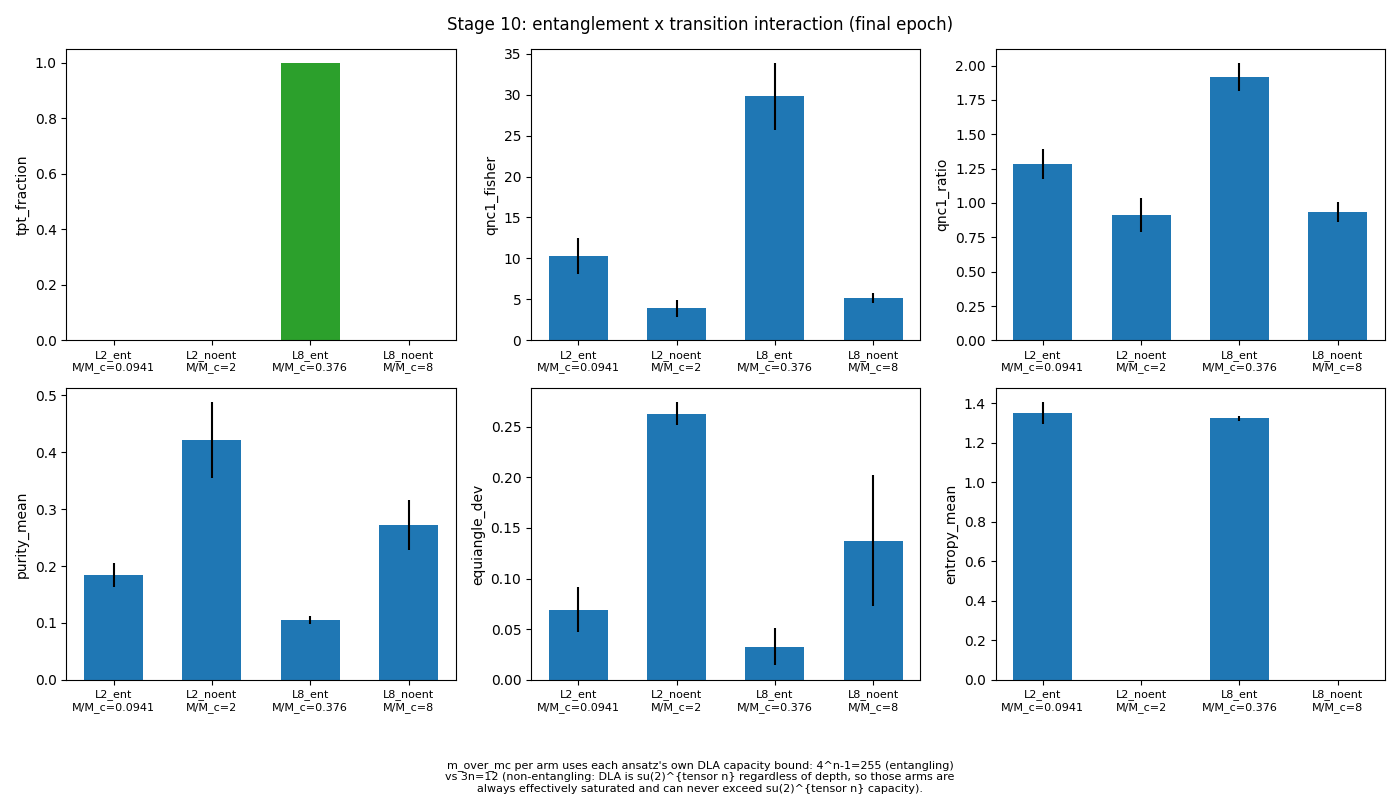
\includegraphics[width=\linewidth]{figures/fig09_ablation_bounds.png}
\caption{Entanglement ablation: TPT fraction vs.\ parameter count, entangling vs.\ non-entangling ansatz, corrected dynamical-Lie-algebra bounds.}
\label{fig:ablation}
\end{figure}

\begin{figure}[h]
\centering
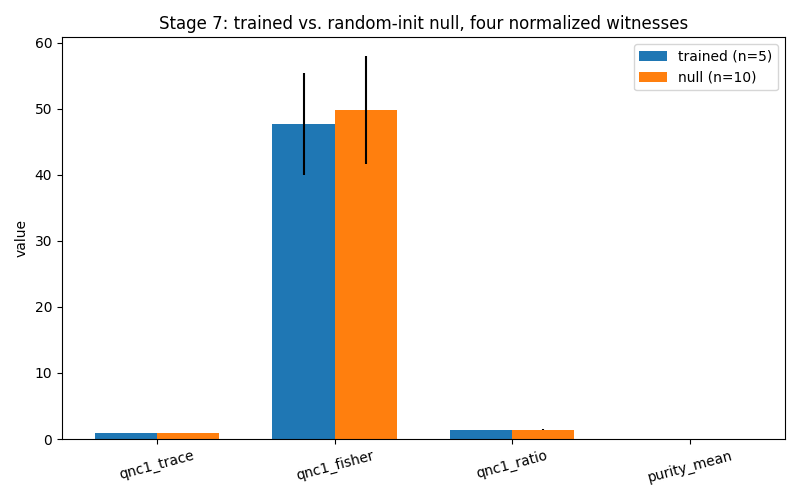
\includegraphics[width=\linewidth]{figures/fig10_four_witness_comparison.png}
\caption{Four normalized collapse witnesses, trained vs.\ untrained null, 2-class anchor.}
\label{fig:fourwitness}
\end{figure}

\begin{figure}[h]
\centering
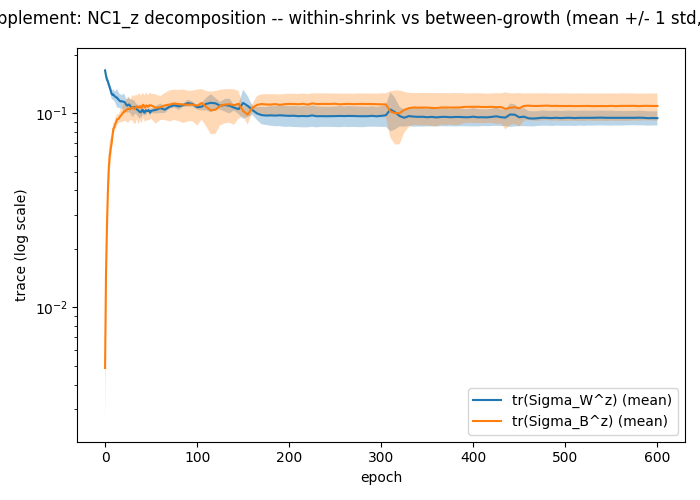
\includegraphics[width=\linewidth]{figures/fig11_nc1z_decomposition.png}
\caption{$\mathrm{tr}(\Sigma_W^z)$ and $\mathrm{tr}(\Sigma_B^z)$ vs.\ epoch, 4-qubit $L{=}8$ anchor.}
\label{fig:nc1zdecomp}
\end{figure}

\begin{figure}[h]
\centering
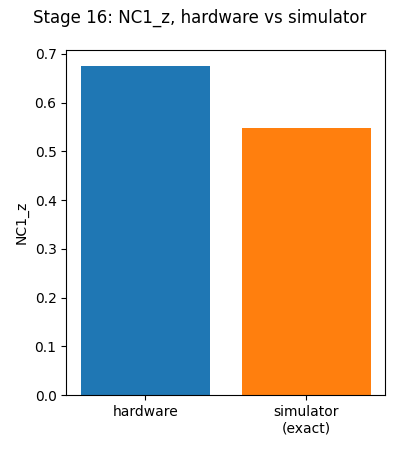
\includegraphics[width=\linewidth]{figures/fig12_nc1z_hw_vs_sim.png}
\caption{$\mathrm{NC1}_z$, hardware (\texttt{ibm\_marrakesh}) vs.\ exact simulator, bar comparison.}
\label{fig:hwbar}
\end{figure}

\end{appendices}

\end{document}
